\documentclass{article}


\usepackage{PRIMEarxiv}

\usepackage[utf8]{inputenc} % allow utf-8 input
\usepackage[T1]{fontenc}    % use 8-bit T1 fonts
\usepackage{hyperref}       % hyperlinks
\usepackage{url}            % simple URL typesetting
\usepackage{booktabs}       % professional-quality tables
\usepackage{amsfonts}       % blackboard math symbols
\usepackage{nicefrac}       % compact symbols for 1/2, etc.
\usepackage{microtype}      % microtypography
\usepackage{lipsum}
\usepackage{fancyhdr}       % header
\usepackage{graphicx}       % graphics
\usepackage[numbers]{natbib}
\graphicspath{{images/}}     % organize your images and other figures under media/ folder
\usepackage{amsmath}
\usepackage{amsfonts}
\usepackage{cancel}
\usepackage{xcolor}
\usepackage{caption}
\usepackage{subcaption}
\usepackage{algorithm2e}

\newcommand{\pygenn}{{PyGeNN }}
\newcommand{\genn}{{GeNN }}
\newcommand\note[1]{\textcolor{red}{(~#1~)}}

%Header
\pagestyle{fancy}
\thispagestyle{empty}
\rhead{ \textit{ }} 

% Update your Headers here
\fancyhead[LO]{Accelerated dendritic micro-circuits}
% \fancyhead[RE]{Firstauthor and Secondauthor} % Firstauthor et al. if more than 2 - must use \documentclass[twoside]{article}



  
%% Title
\title{Accelerated Dendritic Micro-Circuits
%%%% Cite as
%%%% Update your official citation here when published 
\thanks{\textit{\underline{Citation}}: 
\textbf{Authors. Title. Pages.... DOI:000000/11111.}} 
}

\author{
  Author1, Author2 \\
  Affiliation \\
  Univ \\
  City\\
  \texttt{\{Author1, Author2\}email@email} \\
  %% examples of more authors
   \And
  Author3 \\
  Affiliation \\
  Univ \\
  City\\
  \texttt{email@email} \\
  %% \AND
  %% Coauthor \\
  %% Affiliation \\
  %% Address \\
  %% \texttt{email} \\
  %% \And
  %% Coauthor \\
  %% Affiliation \\
  %% Address \\
  %% \texttt{email} \\
  %% \And
  %% Coauthor \\
  %% Affiliation \\
  %% Address \\
  %% \texttt{email} \\
}


\begin{document}
\maketitle


\begin{abstract}
Recently, researchers have found that neuronal circuits could perform bio-plausible deep learning. 
Simulating such complex networks typically takes extensive computational resources. 
Fortunately, the elements in the network can be decoupled and simulated in parallel.
Graphics Processing Units (GPUs) are a good fit in this situation as they posses multiple (simple) compute units which can execute programs in parallel.
Our GPU-based implementation is \note{how much} faster than the standard (CPU).
We have also generated event-driven implementations of the algorithms though they have not proven to be faster.

\end{abstract}


% keywords can be removed
\keywords{First keyword \and Second keyword \and More}


\section{Introduction}
Modern machine learning has seen the resurgence of neural networks, particularly Deep Neural Networks (DNNs). 
These have shown great power and flexibility to solve multiple problems, such as image recognition, natural language processing, forecasting, music generation, etc.~\citep{deep-learning-book,deep-learning-nature}
Deep learning, the process of training DNNs, is commonly done via the the back-propagation (BP) of errors algorithm~\cite{backprop}.
One issue with standard DNNs is the computational power they require to do both training and inference.

Finding bio-plausible \note{/ compatible} algorithms which can produce as good performance for neural networks as BP is the focus of intense and interesting research.
Furthermore, because bio-plausible \note{spiking} neuron and synapse simulations can be very efficiently in hardware, finding an algorithm to train deep networks would be of great use for energy-efficient machine learning.
\citeauthor{bengio_bio_deep} explored the interpretation of a classical \note{`neuroscience'} learning algorithm, Spike-Timing-Dependent Plasticity (STDP)~\citep{stdp} but, in the context of deep learning~\citep{bengio_bio_deep}.
The Authors propose that STDP could be performing an approximate stochastic gradient descent per layer.
Using a variant of Target Propagation~\cite{target-prop}, \citeauthor{lee_diff_prop} show that discrete transmission of `information' can be used to train DNNs~\citep{lee_diff_prop}.
Importantly, these algorithms require two phases for the neurons in the network


Starting from a neuroscience perspective \note{or just Europe :P} , \citeauthor{urbanczik} proposed a learning rule which makes use of different compartments in neurons to transmit errors between `layers'~\cite{urbanczik}, and thus, possibly train DNNs.
Recently, \citeauthor{sacramento}, showed that their \note{architecture and} algorithm could be used to train DNNs as it is an approximation to BP~\citep{sacramento}.
This algorithm has sparked much interest since the modeling was done with biological plausibility constraints.
\citeauthor{cartiglia_snn_prop} describe a spike-based learning algorithm that could be used to transmit errors on a DNN~\citep{cartiglia_snn_prop}; since it uses spikes for the communication between neurons, it could be deployed in neuromorphic hardware.
Distinctly \note{ideally?}, these algorithms do not require distinct phases of neurons to perform learning, making them ideal for robotics or continual learning.


\note{What else should we put here? Are we going to implement the new version?}

\section{Accelerating cortical microcircuits}
\label{sec:accelerating-microcircuit}
The cortical micro circuit (CMC) we'll be simulating is the one proposed by \citeauthor{sacramento} (Figure~\ref{fig:micro-circuit}).
In it, signals coming from upper layers when compared with feed-back from inter-neurons generate an error signal to change the efficacy of plastic synapses.
\note{should I do more of a description here?}
Fortunately, elements in the circuit, i.e. synapses and neurons, can be simulated in parallel \note{although first synapses, then neurons} which allows the use of hardware acceleration to reduce the computation time.

\begin{figure}[h!bt]
    \centering
    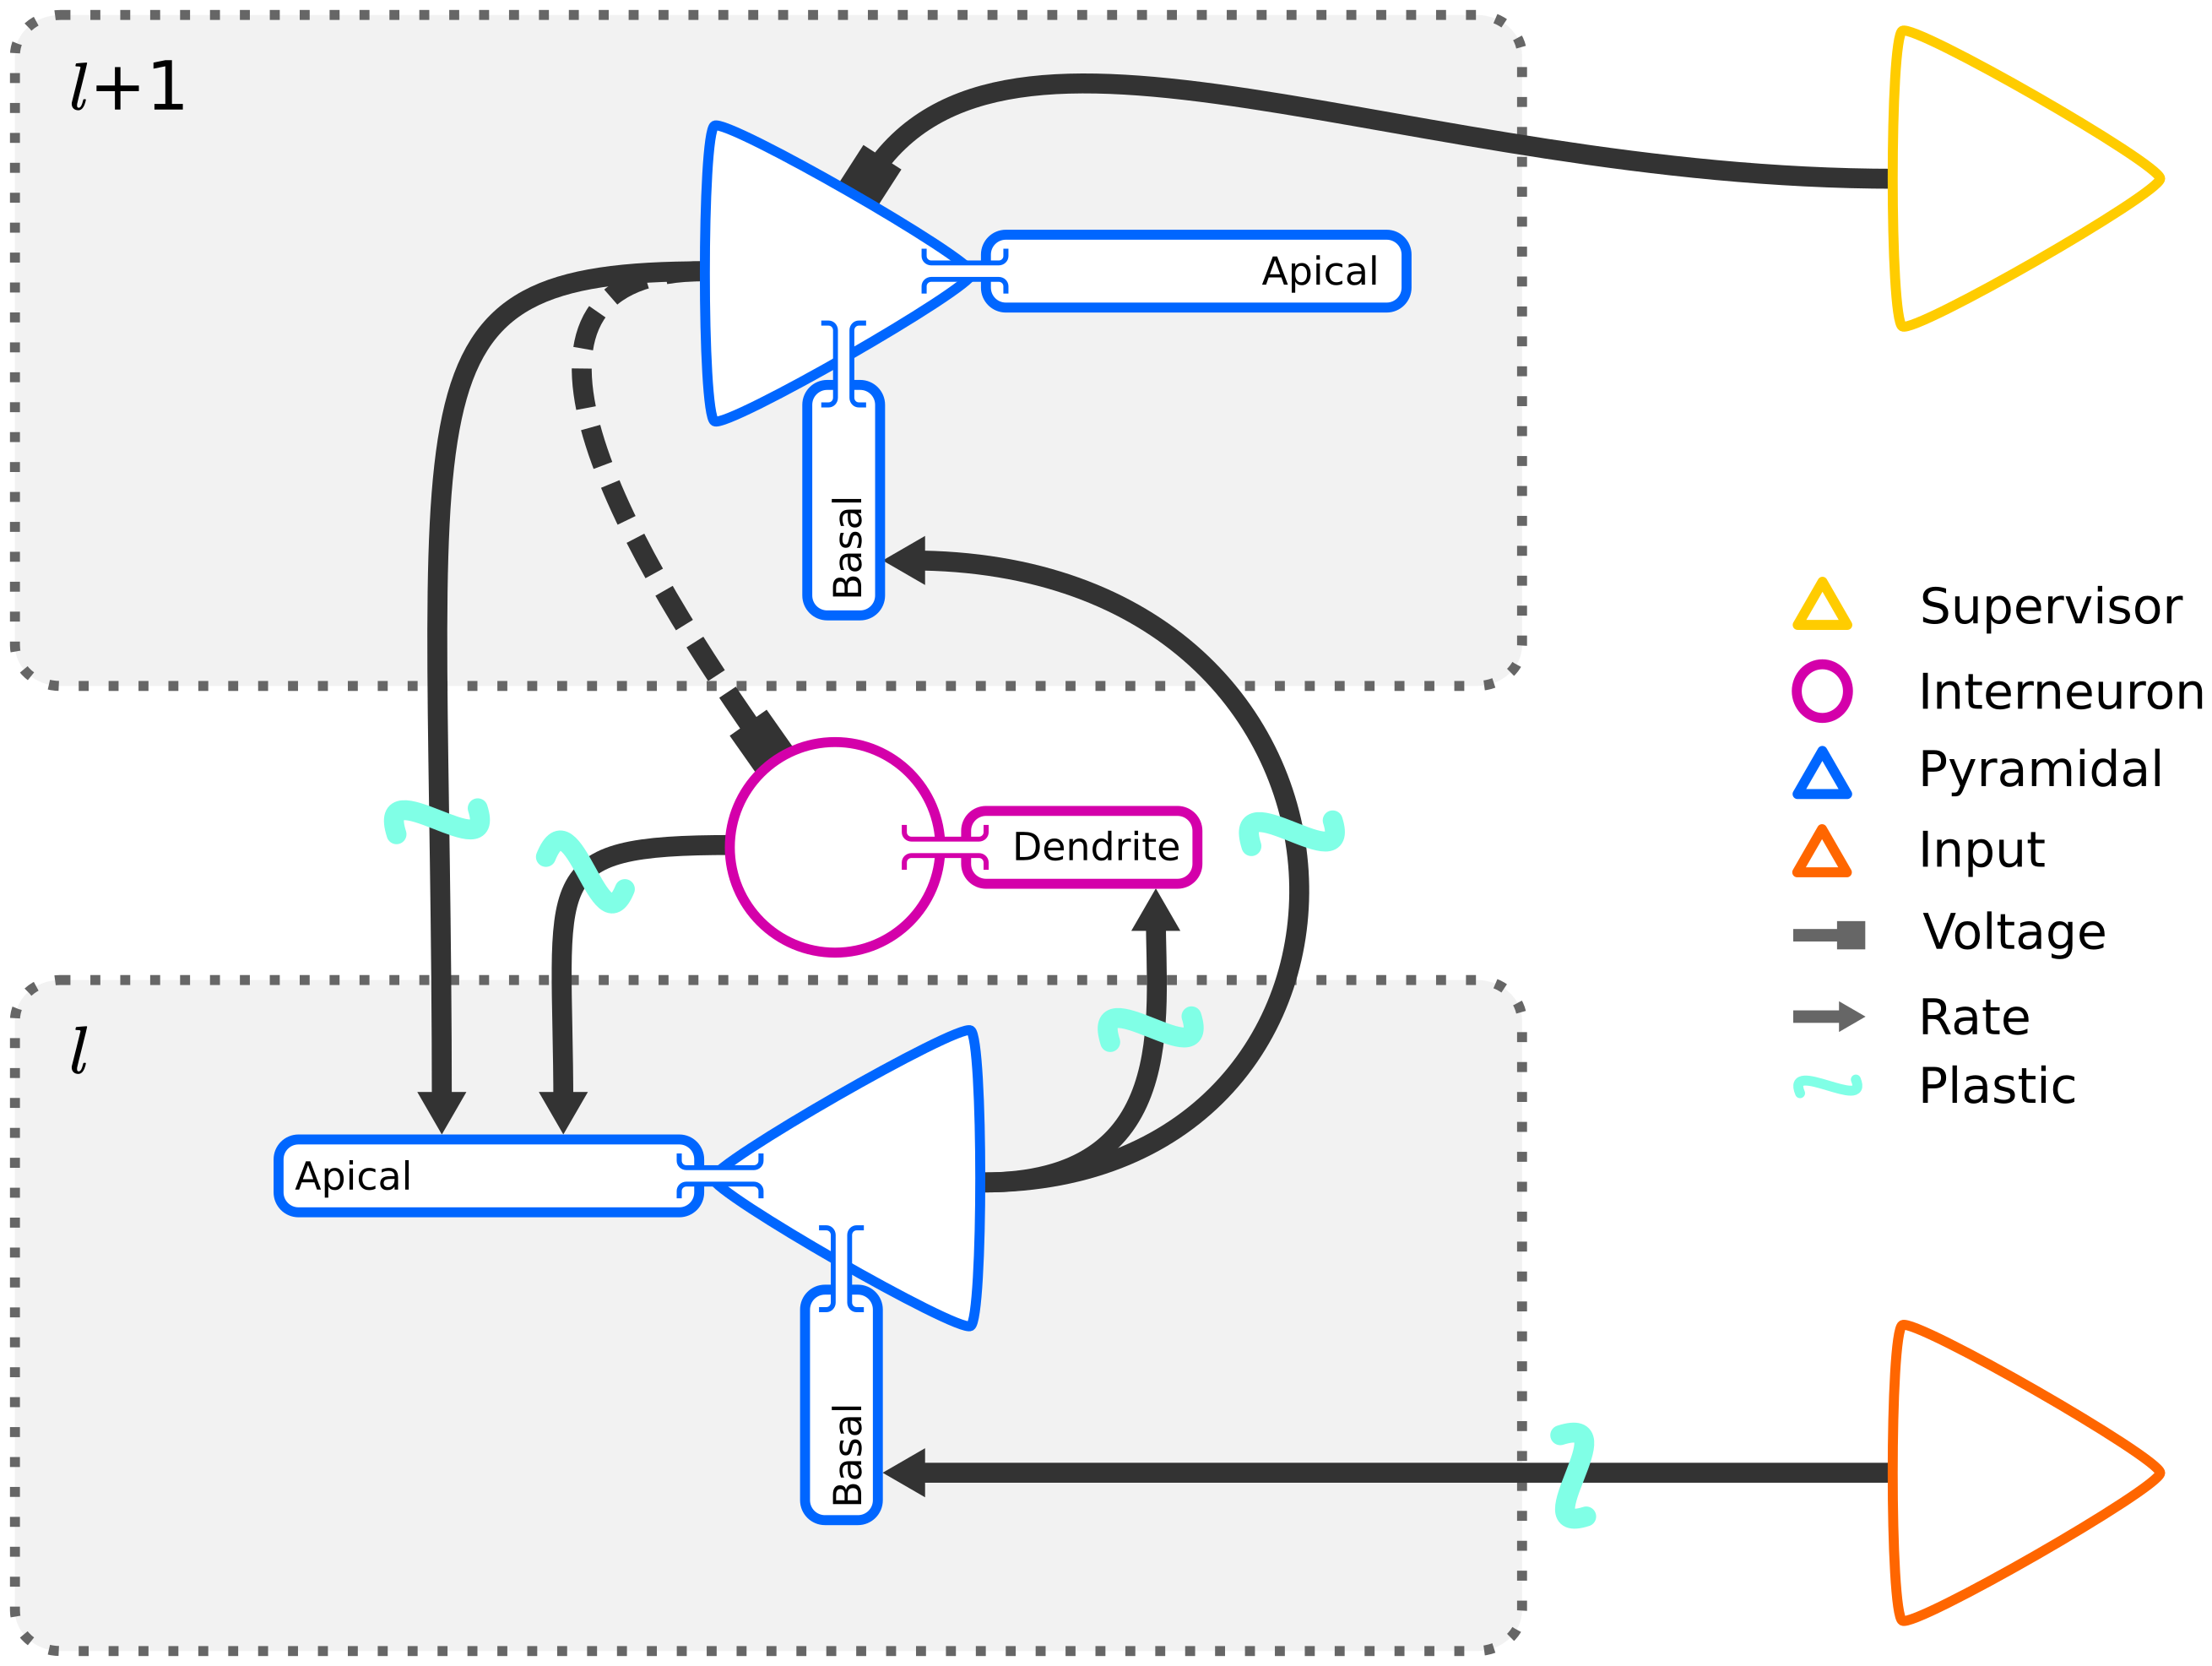
\includegraphics[width=0.5\textwidth]{neuron_models.png}
    \caption{Cortical micro circuit}
    \label{fig:micro-circuit}
\end{figure}

\note{TODO: add short math description of the model to reference later}
This CMC is rate-based, thus each neuron sends a rate value out every \note{time?} simulation step. 
Pyramidal neurons have two distinct dendriticcompartments \note{although the voltage link could be seen as an extra compartment?}
\begin{equation}
    x,y,z
\end{equation}
and integrate their inputs 
\begin{equation}
    x,y,z
\end{equation}

Similarly, inter-neurons have a single dendritic compartment \note{although the voltage link could be seen as an extra compartment?}
\begin{equation}
    x,y,z
\end{equation}
and add inputs 
\begin{equation}
    x,y,z
\end{equation}

Static synapses are basically weight multiplies and plastic synapses are governed by
\begin{equation}
    x,y,z
\end{equation}
Note that when plasticity is not active, plastic synapses behave just like static ones, i.e. they just multiply the rate by the weight.

The resurgence and success of recent DNNs has been, partly, due to modern computing hardware.
In particular, GPUs have played a key role since their parallel architecture \note{is not particularly a good fit but it is sufficient} is compatible with the idea of neural networks, i.e. multiple independent units \note{with little computational power}.
\citeauthor{genn} created a framework [\genn;~\citenum{genn}] which allows the user to express \note{neuron and synapse} models using a modified C++ syntax and execute them on GPUS without worrying about the complexities of using these accelerators.
Furthermore, \citeauthor{pygenn} have continued to improve usability \note{friendliness?} and now provide Python wrappers via \pygenn~\citep{pygenn}, though C++ is still used to describe model behaviour.

\begin{figure}[h!bt]
    \centering
    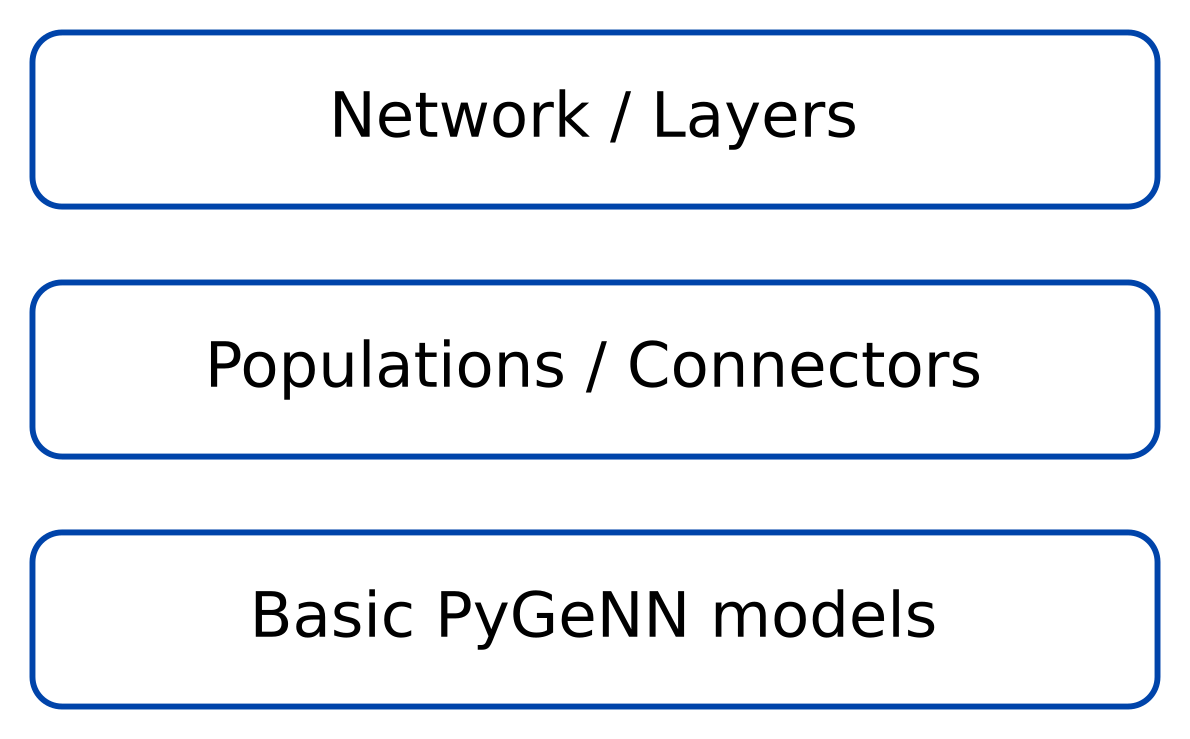
\includegraphics[width=0.3\textwidth]{abstraction_layers.png}
    \caption{Software abstractions}
    \label{fig:abstractions}
\end{figure}

In this work we have generated neuron and synapse models required for the implementation of the cortical micro circuit using \pygenn (Figure~\ref{fig:abstractions}). 
Additionally, we created abstractions of the models at the Population and Connection levels, this reduces necessary coding and ensures correctness of model initialization. 
On top of these, we built Layer and Network level abstractions to further reduce required coding, which lead to the possibility to use a small description to generate a full network.

\section{Results}
\subsection{Continuous evaluation}

Initially, we ported the models to \pygenn and checked that they work correctly using three test tasks.
\begin{itemize}
    \item {The First task consist of simulating a \note{small/tiny} network and recording its input-output, this will generate training and validation sets.
    Afterwards, we train a network with the same structure, but different weights, to generate the desired outputs given the recorded inputs.}
    \item {The Second task requires to classify input images of bars \note{vertical, horizontal, 45 and 135 degrees}. 
    Each input pixel is represented by an input neuron and each classification by an active output neuron.}
    \item {Similarly, the Third task, consists of classifying dots depending on where they fall in a Yin Yang symbol~\cite{yinyang_dataset}.}
\end{itemize}

Figure~\ref{fig:std-test-tasks} shows the performance of the \genn-based implementation of the CMC; all the tasks have been solved using our implementation.
For the first task, we check the mean squared error (MSE) of the trained network vs a target validation signal (Figure~\ref{fig:std-mimic-validation}) over the training epochs.
The two last plots (Figures~\ref{fig:std-bars-validation} and \ref{fig:std-yinyang-validation}) present the accuracy over epochs on validation sets for the bars and Yin Yang datasets, respectively.

\begin{figure}[hbt]
    \centering
    \begin{subfigure}[b]{0.33\textwidth}
        \centering 
        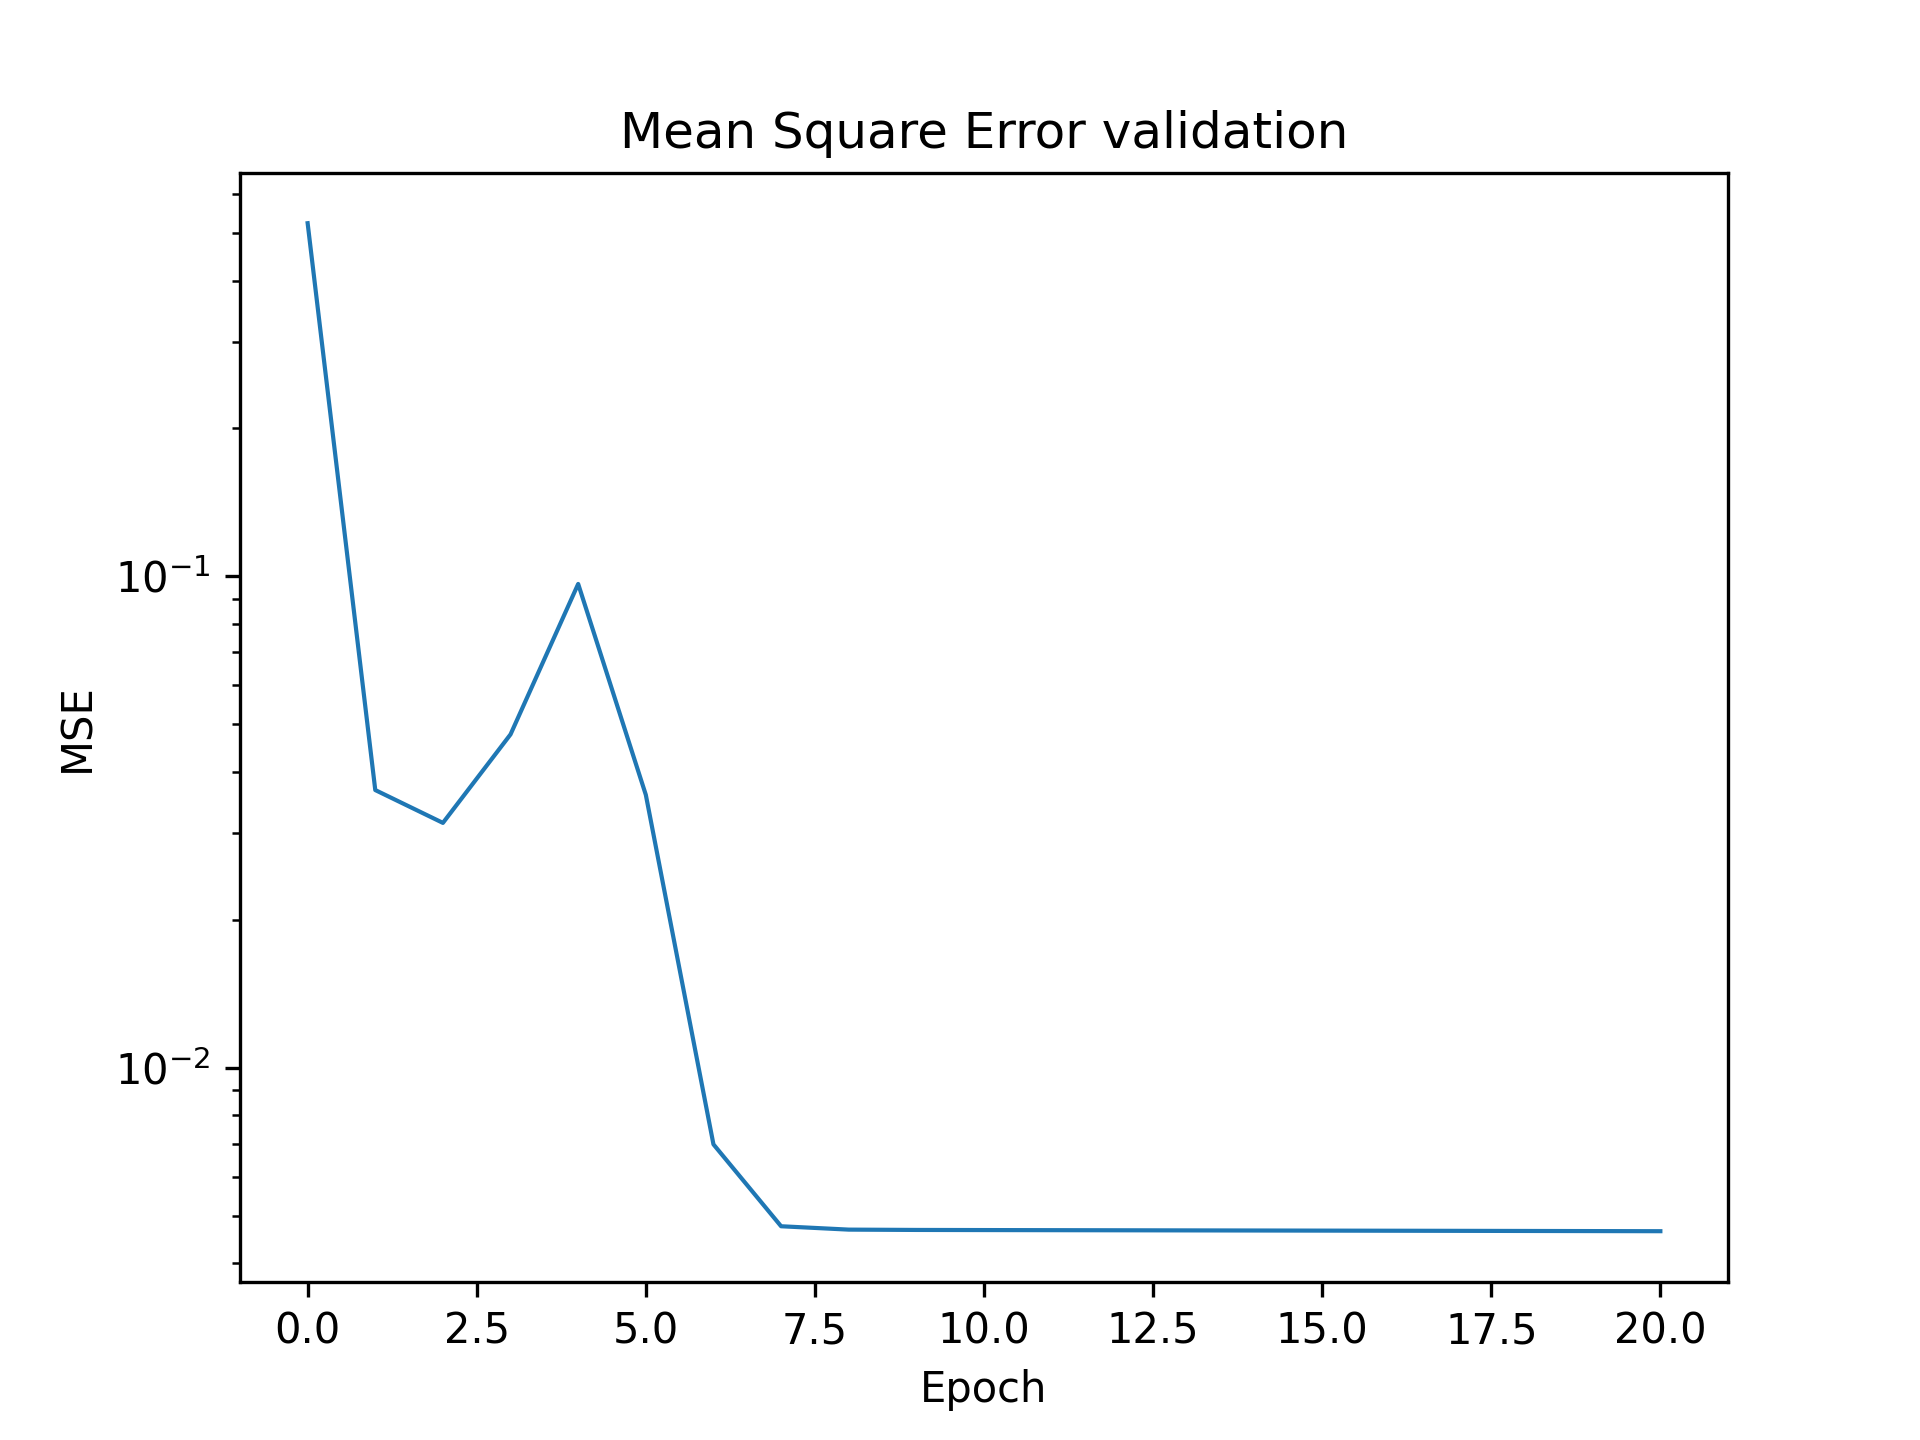
\includegraphics[width=\textwidth,trim={0 0 0 1.2cm},clip]{std_mimic_mse_validation.png}
        \caption{}
        \label{fig:std-mimic-validation}
    \end{subfigure}
    \hfill
    \begin{subfigure}[b]{0.33\textwidth}
        \centering 
        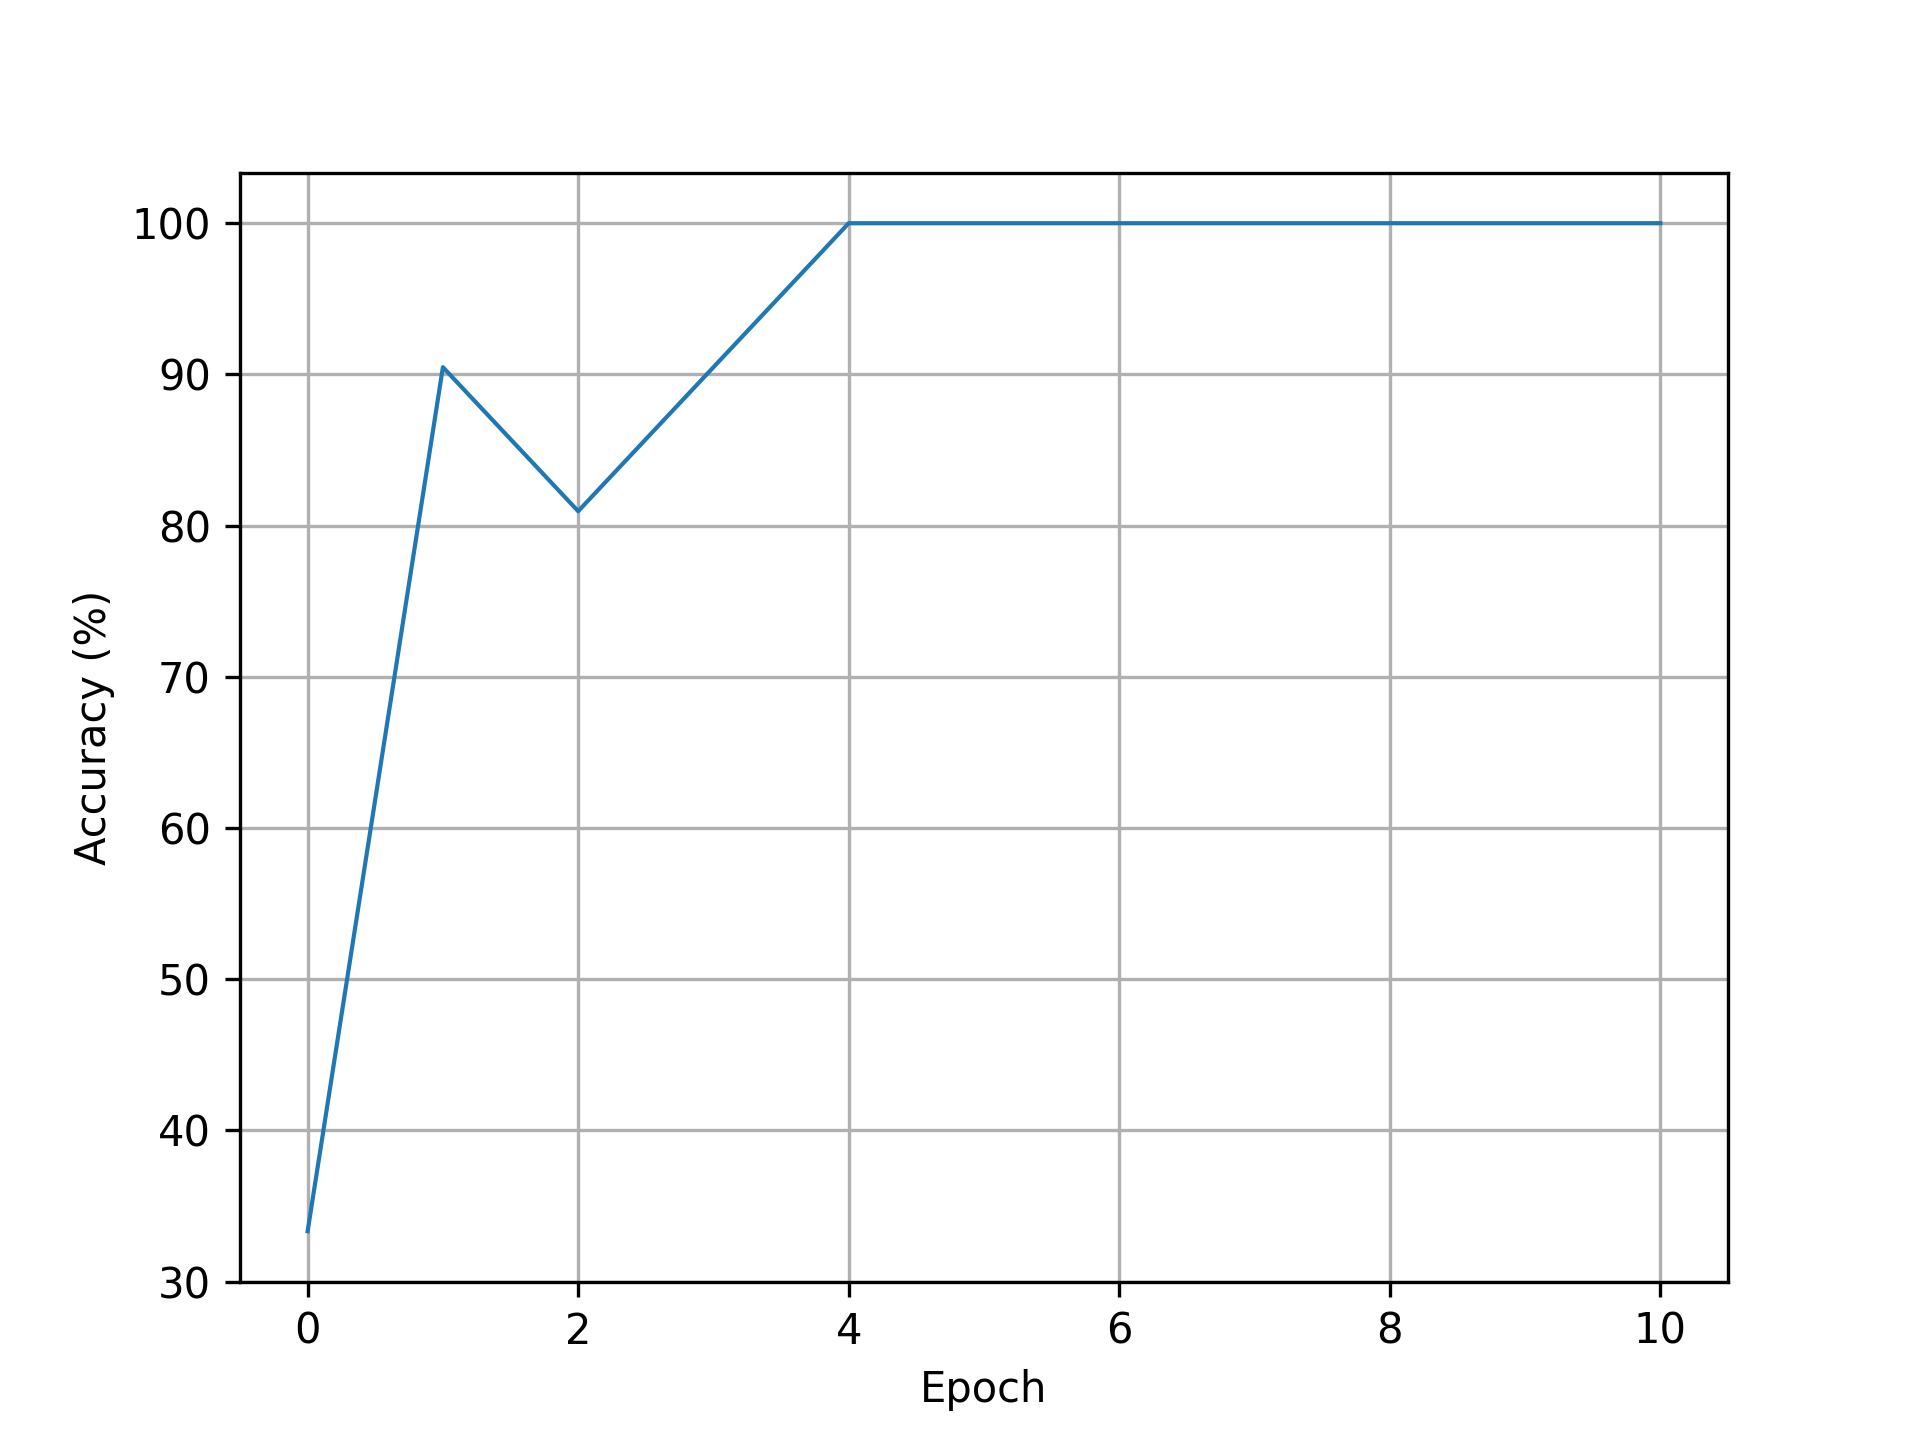
\includegraphics[width=\textwidth]{std_bars_accuracy.png} \caption{}
        \label{fig:std-bars-validation}
    \end{subfigure}
    \hfill
    \begin{subfigure}[b]{0.33\textwidth}
        \centering 
        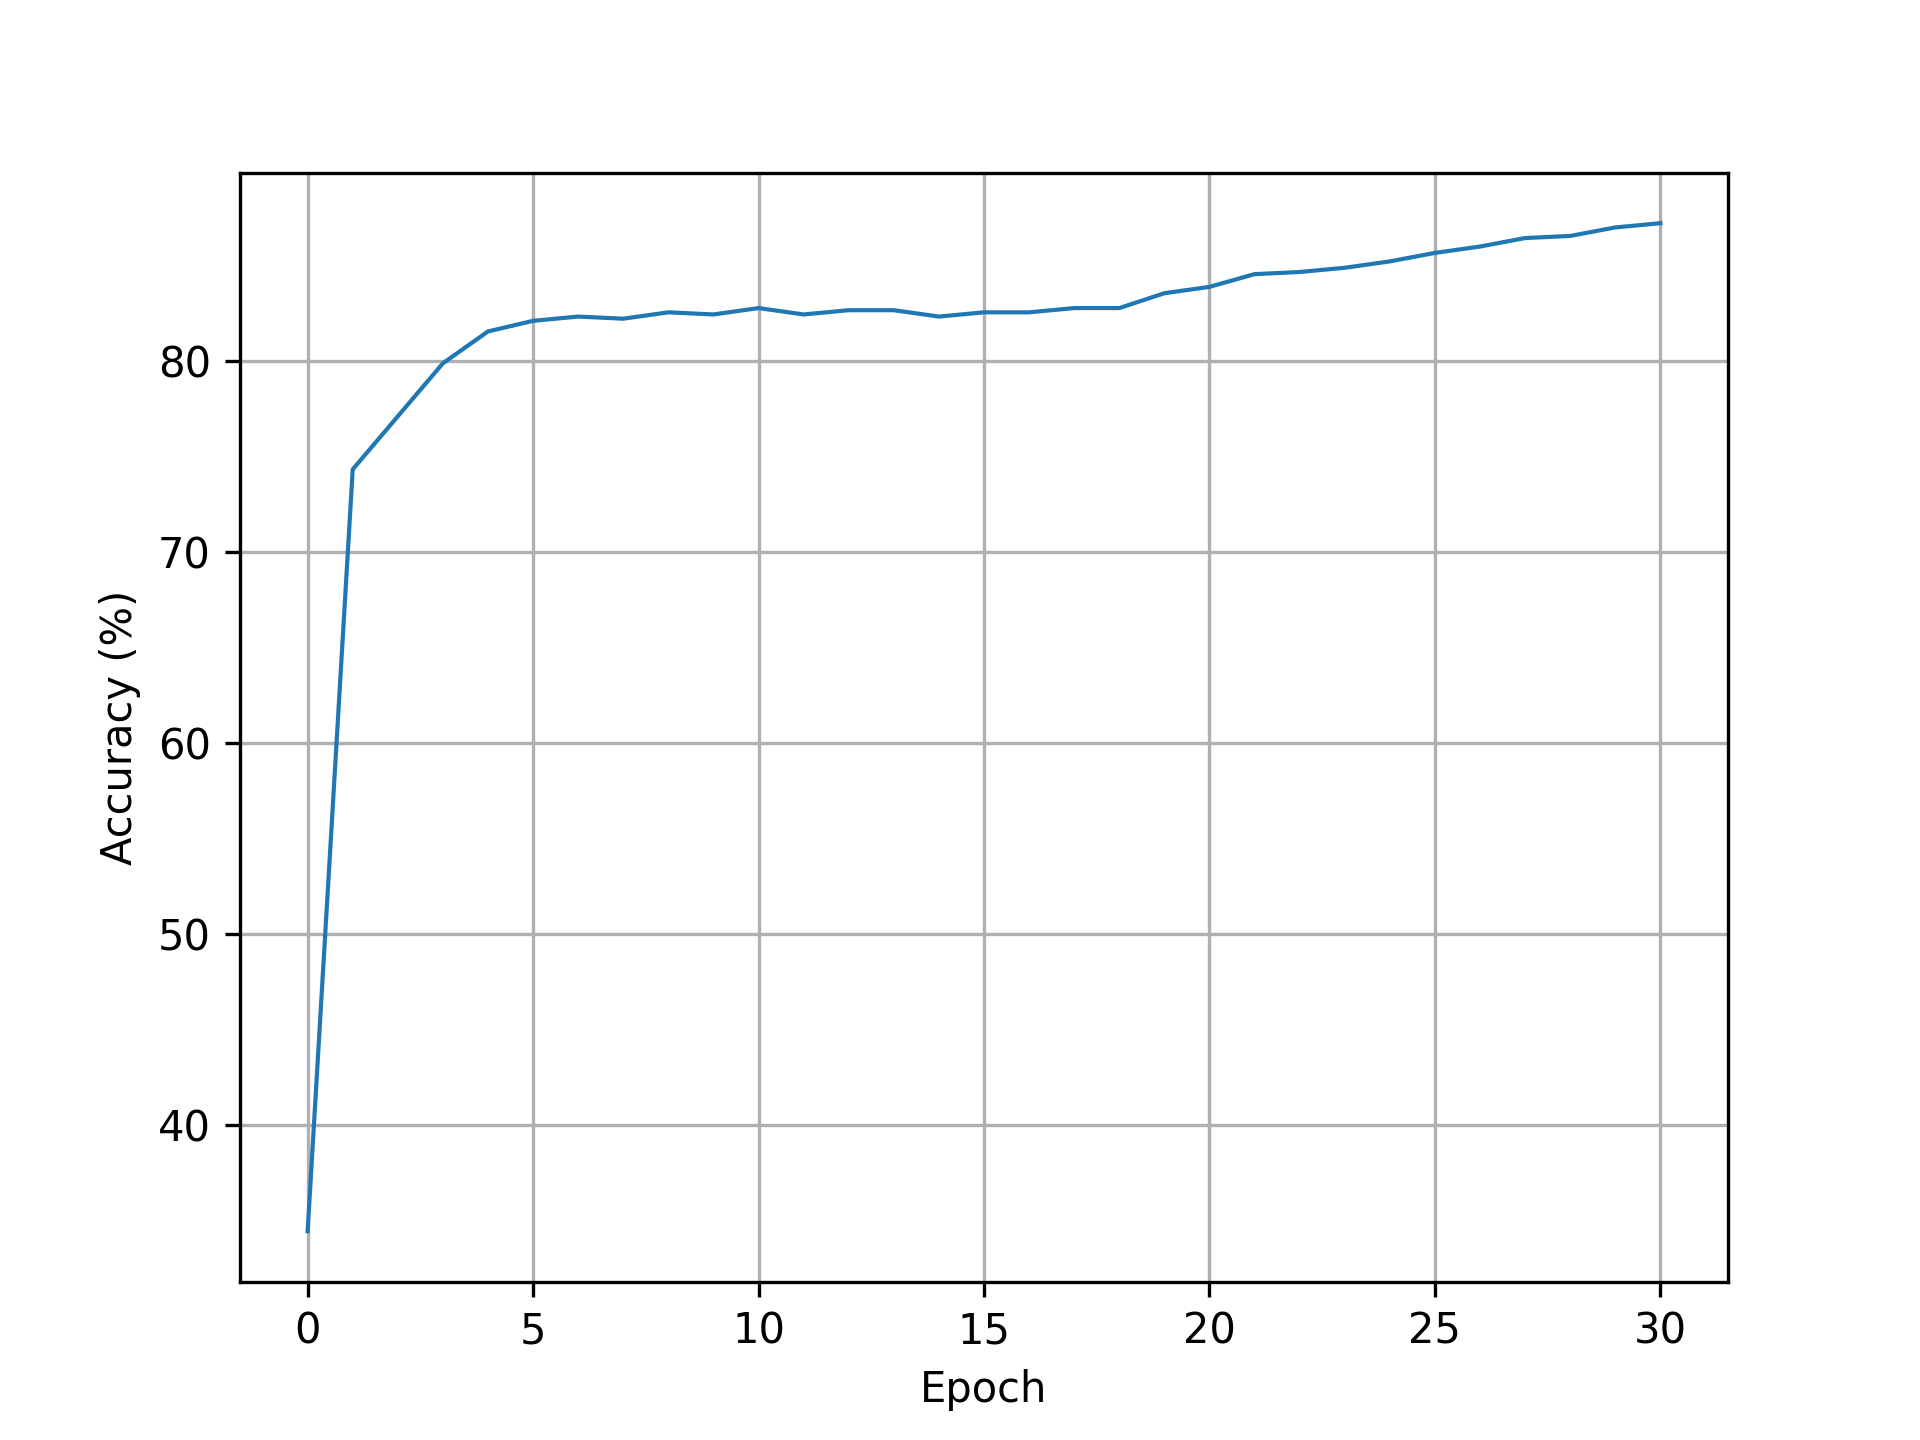
\includegraphics[width=\textwidth]{std_yinyang_accuracy.png}
        \caption{}
        \label{fig:std-yinyang-validation}
    \end{subfigure}
    \caption{Test tasks. Mimic network, Bars image classification, Yin Yang dataset classification.}
    \label{fig:std-test-tasks}
\end{figure}

The first and second networks use the soft ReLU activation function for neurons.
The third network uses the Sigmoid activation function, this looks like the only way to keep the activity and weight changes bound so that the network solves the task. 
\note{I think this is the same case for the Numpy version?}



After we checked that the implementation was working correctly, we measured the time it takes to run experiments. 
To test this, we used a 3-layered network (input, hidden and output layers) and executed the network on a computer with an 
\texttt{AMD EPYC 7302 16-Core Processor; 64 GB of DDR4, 2666 Mbps, Samsung RAM; a 1TB NVMe Kingston KC2500 drive; and an NVIDIA GeForce RTX 3080 with 10GB of RAM}. 
We tested using 1500 input samples and an increasing number of neurons in the hidden layer.

\begin{figure}[h]
    \centering
    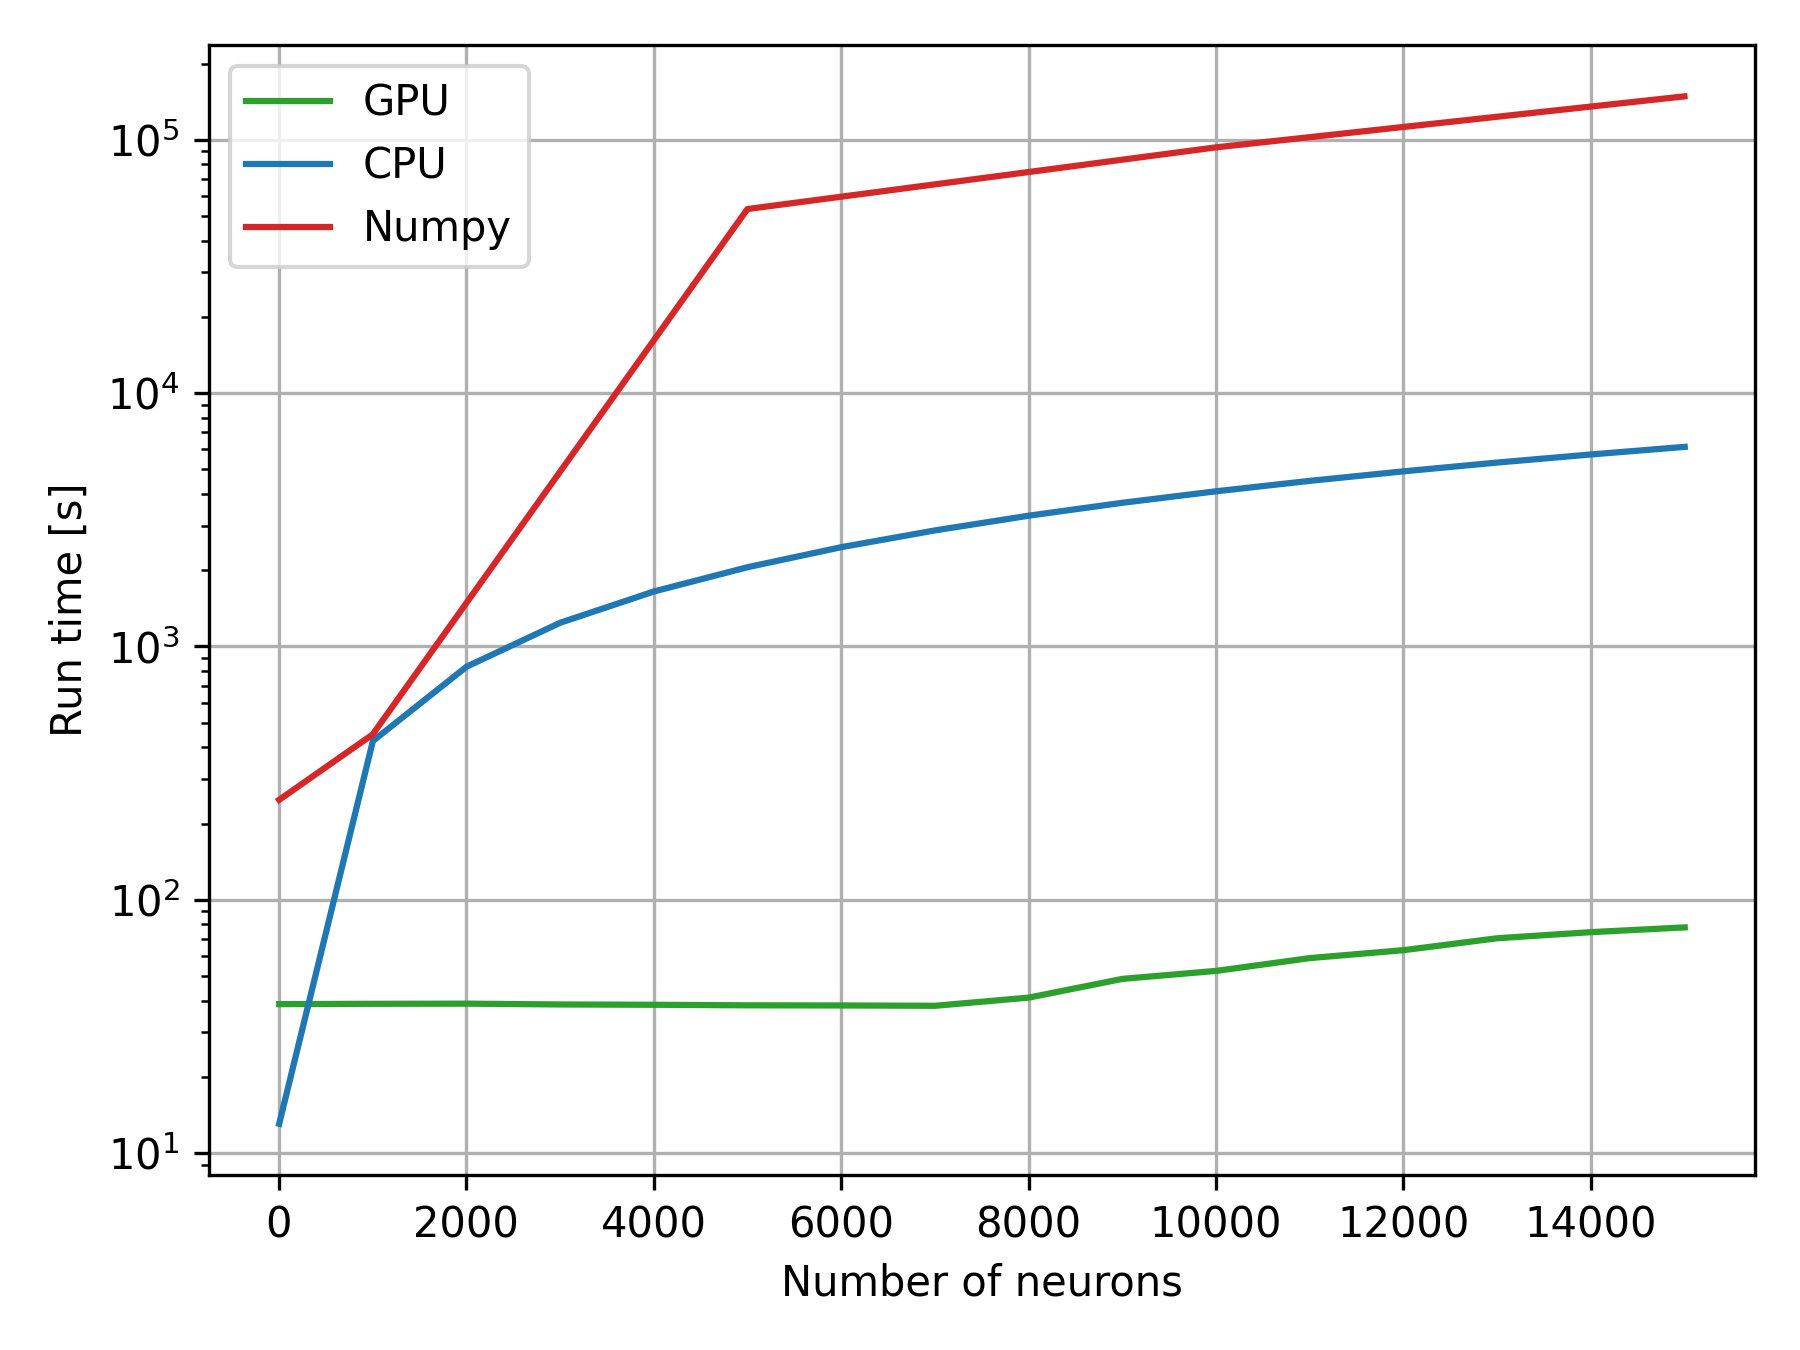
\includegraphics[width=0.5\textwidth]{perf_Numpy_comparison_with_1500_inputs.png}
    \caption{Performance comparison for base algorithm.}
    \label{fig:perf-comparison-basic}
\end{figure}

In Figure~\ref{fig:perf-comparison-basic} we can observe that the Numpy implementation is the slowest; this is likely due to the matrix-oriented computation of the library.
Second comes the CPU-executed version of the \genn ~implementation, for small networks it can even be faster than using a GPU (likely due to data transfers between main RAM and GPU RAM).
Finally, the fastest implementation is the \genn one running on a GPU. 

We then examined computational cost across number of input samples and number of neurons in the hidden layer (Figure~\ref{fig:perf-genn-continuous}).
As expected, as the number of inputs samples increase, the time to run experiments increases, though it seems that the major contributor to computing cost is the number of neurons and, therefore, synapses.

\note{seems like most compute time spent in synapses, in this particular case all-to-all connectivity $O\left(n^2\right)$}

\begin{figure}[h!bt]
    \centering
    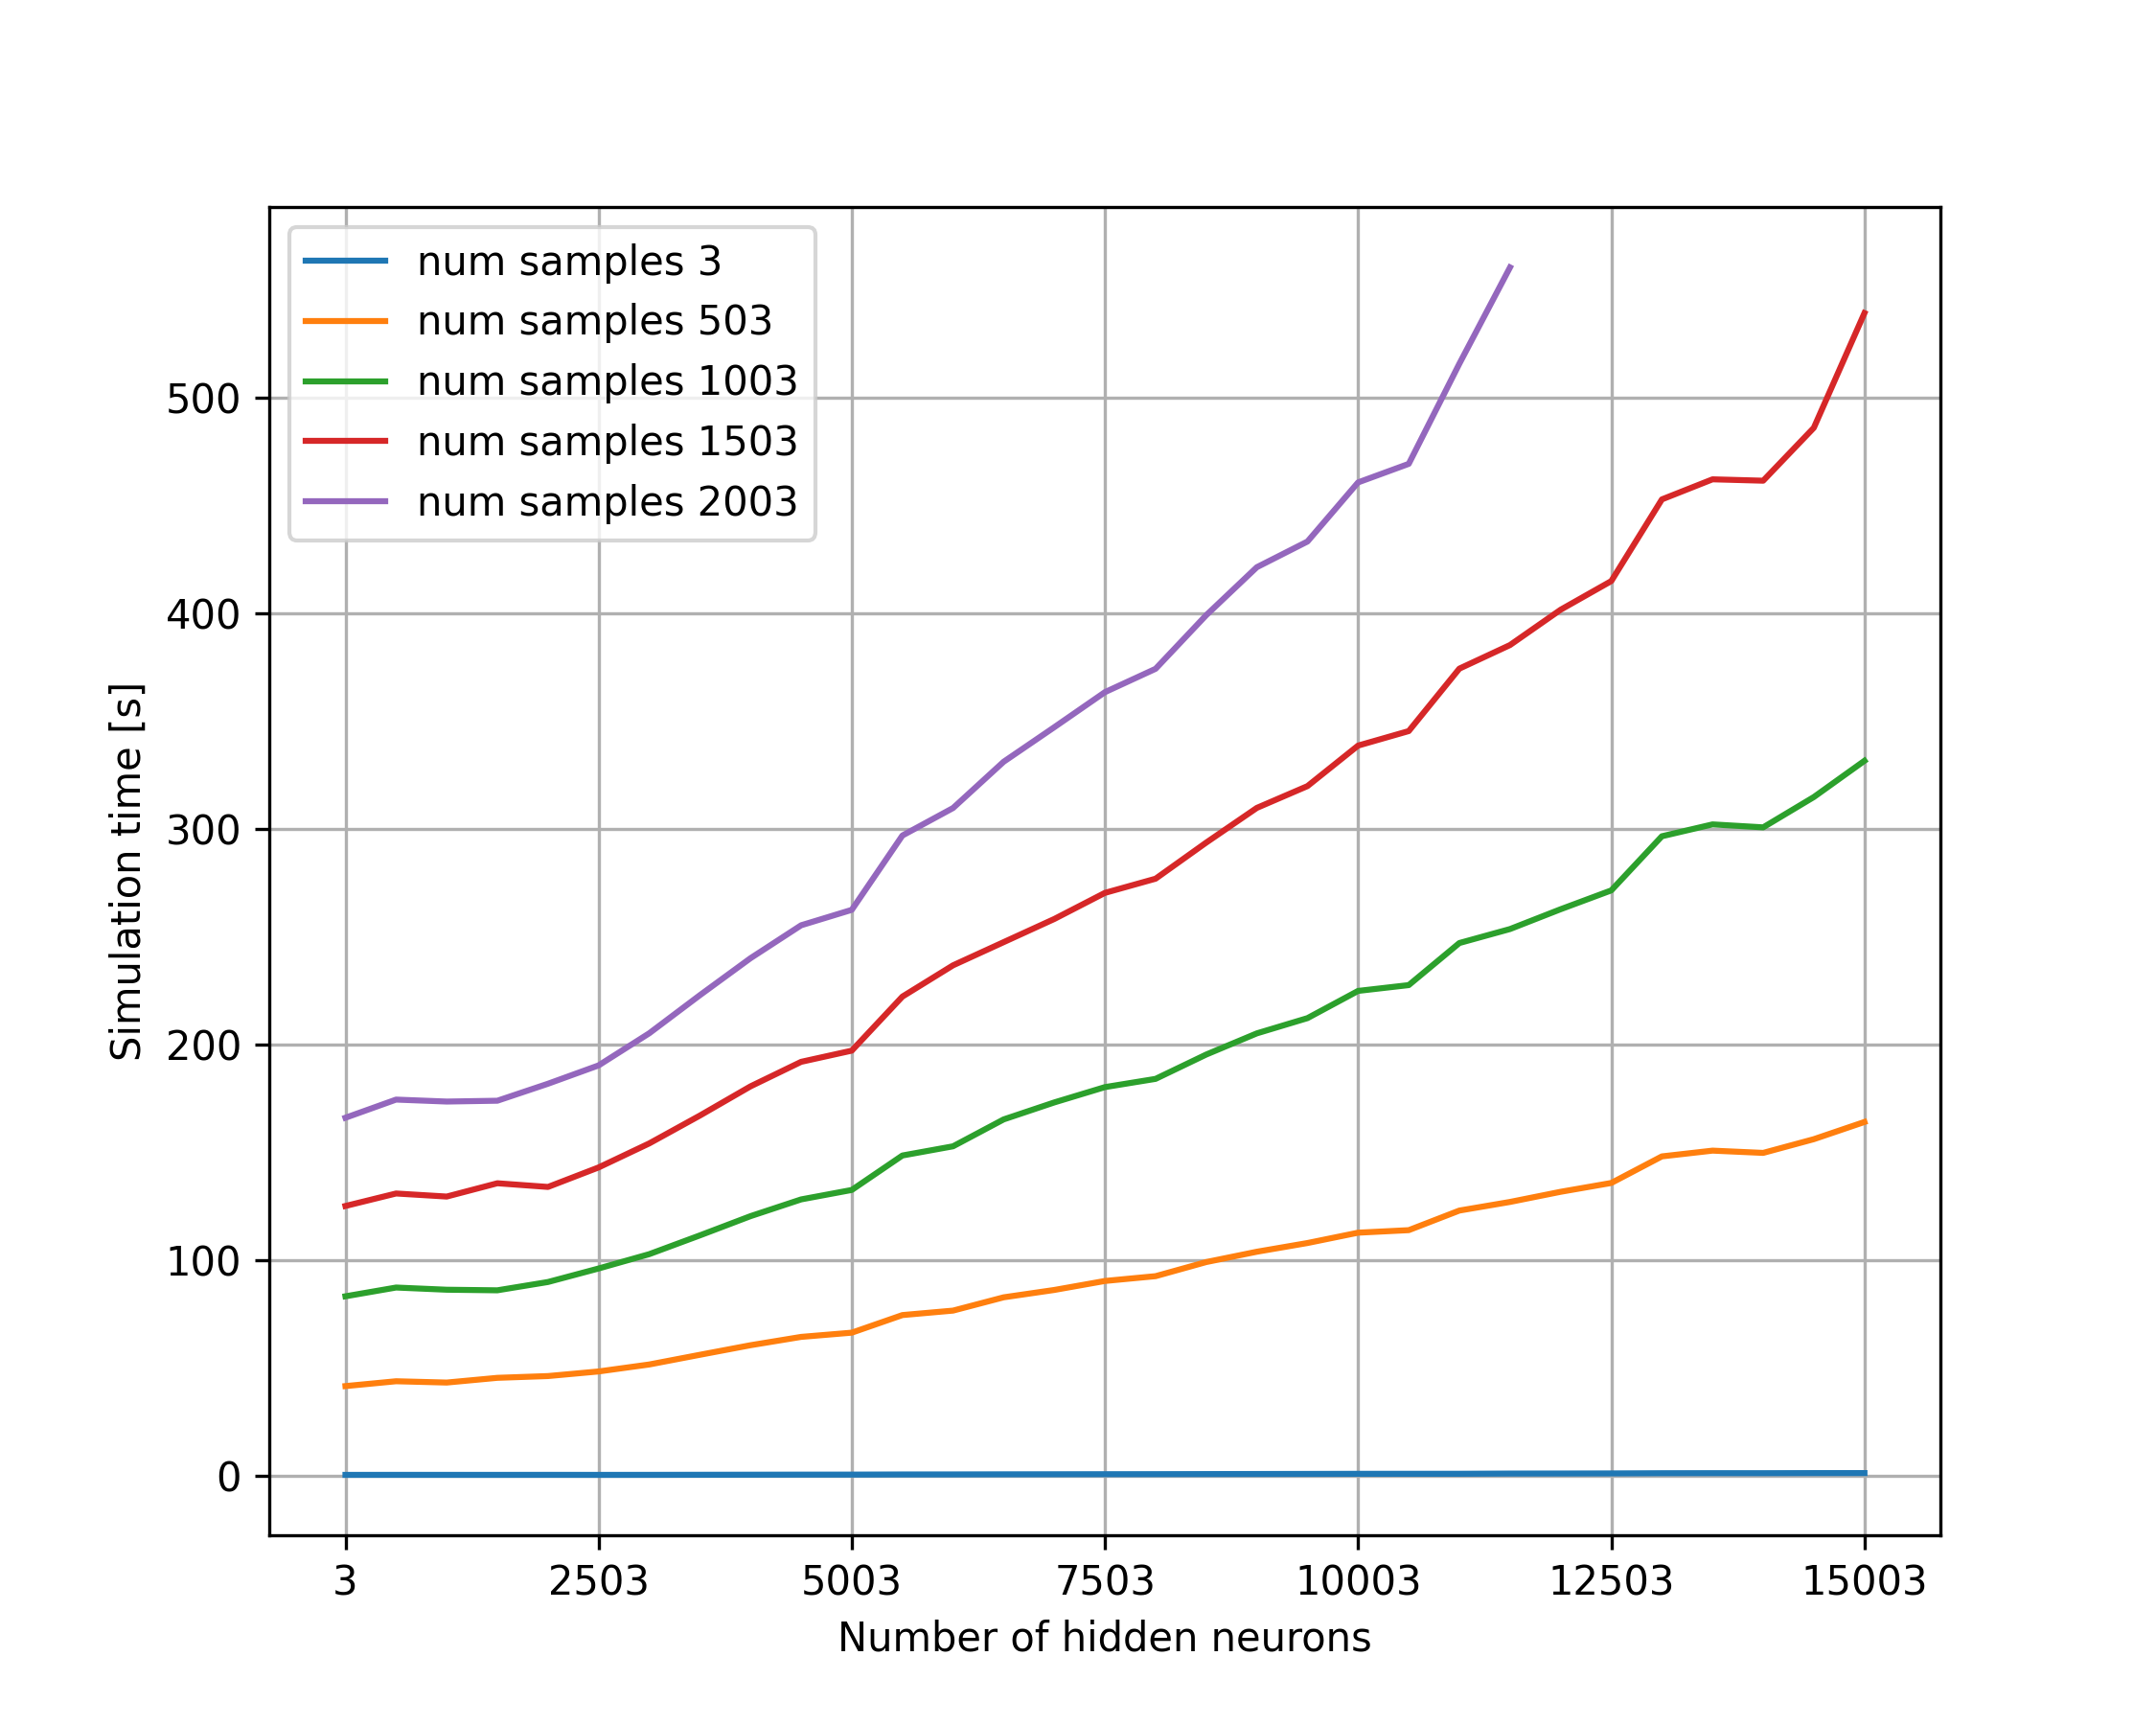
\includegraphics[width=0.5\textwidth]{perf_yinyang_lines.png}
    \caption{Performance for continuous version}
    \label{fig:perf-genn-continuous}
\end{figure}


Rate transmission can be approximated in discrete steps, i.e. events/spikes.
This can also help reduce the computational load to weight changes/training as these would only be evaluated when a spike arrives to the post-synaptic neuron. 
To be able to perform the changes at arbitrary spike times we have to integrate the differential equations of the continuous model \note{ref to eqs}.

\subsection{Event-driven weight changes}
The rate transmitted is multiplied by the connection weight\\
Occurs when a pre-synaptic spike arrives and learning is active\\
Maths\\
\begin{eqnarray}
g_{k+1} &=& g_{k} -\eta \tau_g \left[V_{o} r_{i} \left(\gamma -\frac{\Delta t}{\tau} \right)  + 
\delta_k \gamma \right] \\
\delta_{k+1} &=& -V_{o} r_{i} \gamma  + \delta_k e^{-\Delta t/\tau}
\end{eqnarray}
where $\Delta t = t_{k + 1} - t_k$ and $\gamma = 1 - e^{-\Delta t/\tau}$


\subsection{Fixed Period}
Neurons emit events every T ms, this requires a payload for rate transmission \\

Figure~\ref{fig:fixed-period-rate-example} shows an example of using fixed-period transmission. 
Events are shown as green bars on top of the bottom panel of Figure~\ref{fig:fixed-period-transmission}, in this example events are generated every $5 ms$. 
In this scheme, we only evaluate synapses once every 50 simulation steps $\left(\frac{5 ms}{0.1 ms/step} = 50 step\right)$.



\begin{figure}[h!bt]
    \centering
    \begin{subfigure}[b]{0.6\textwidth}
        \centering 
        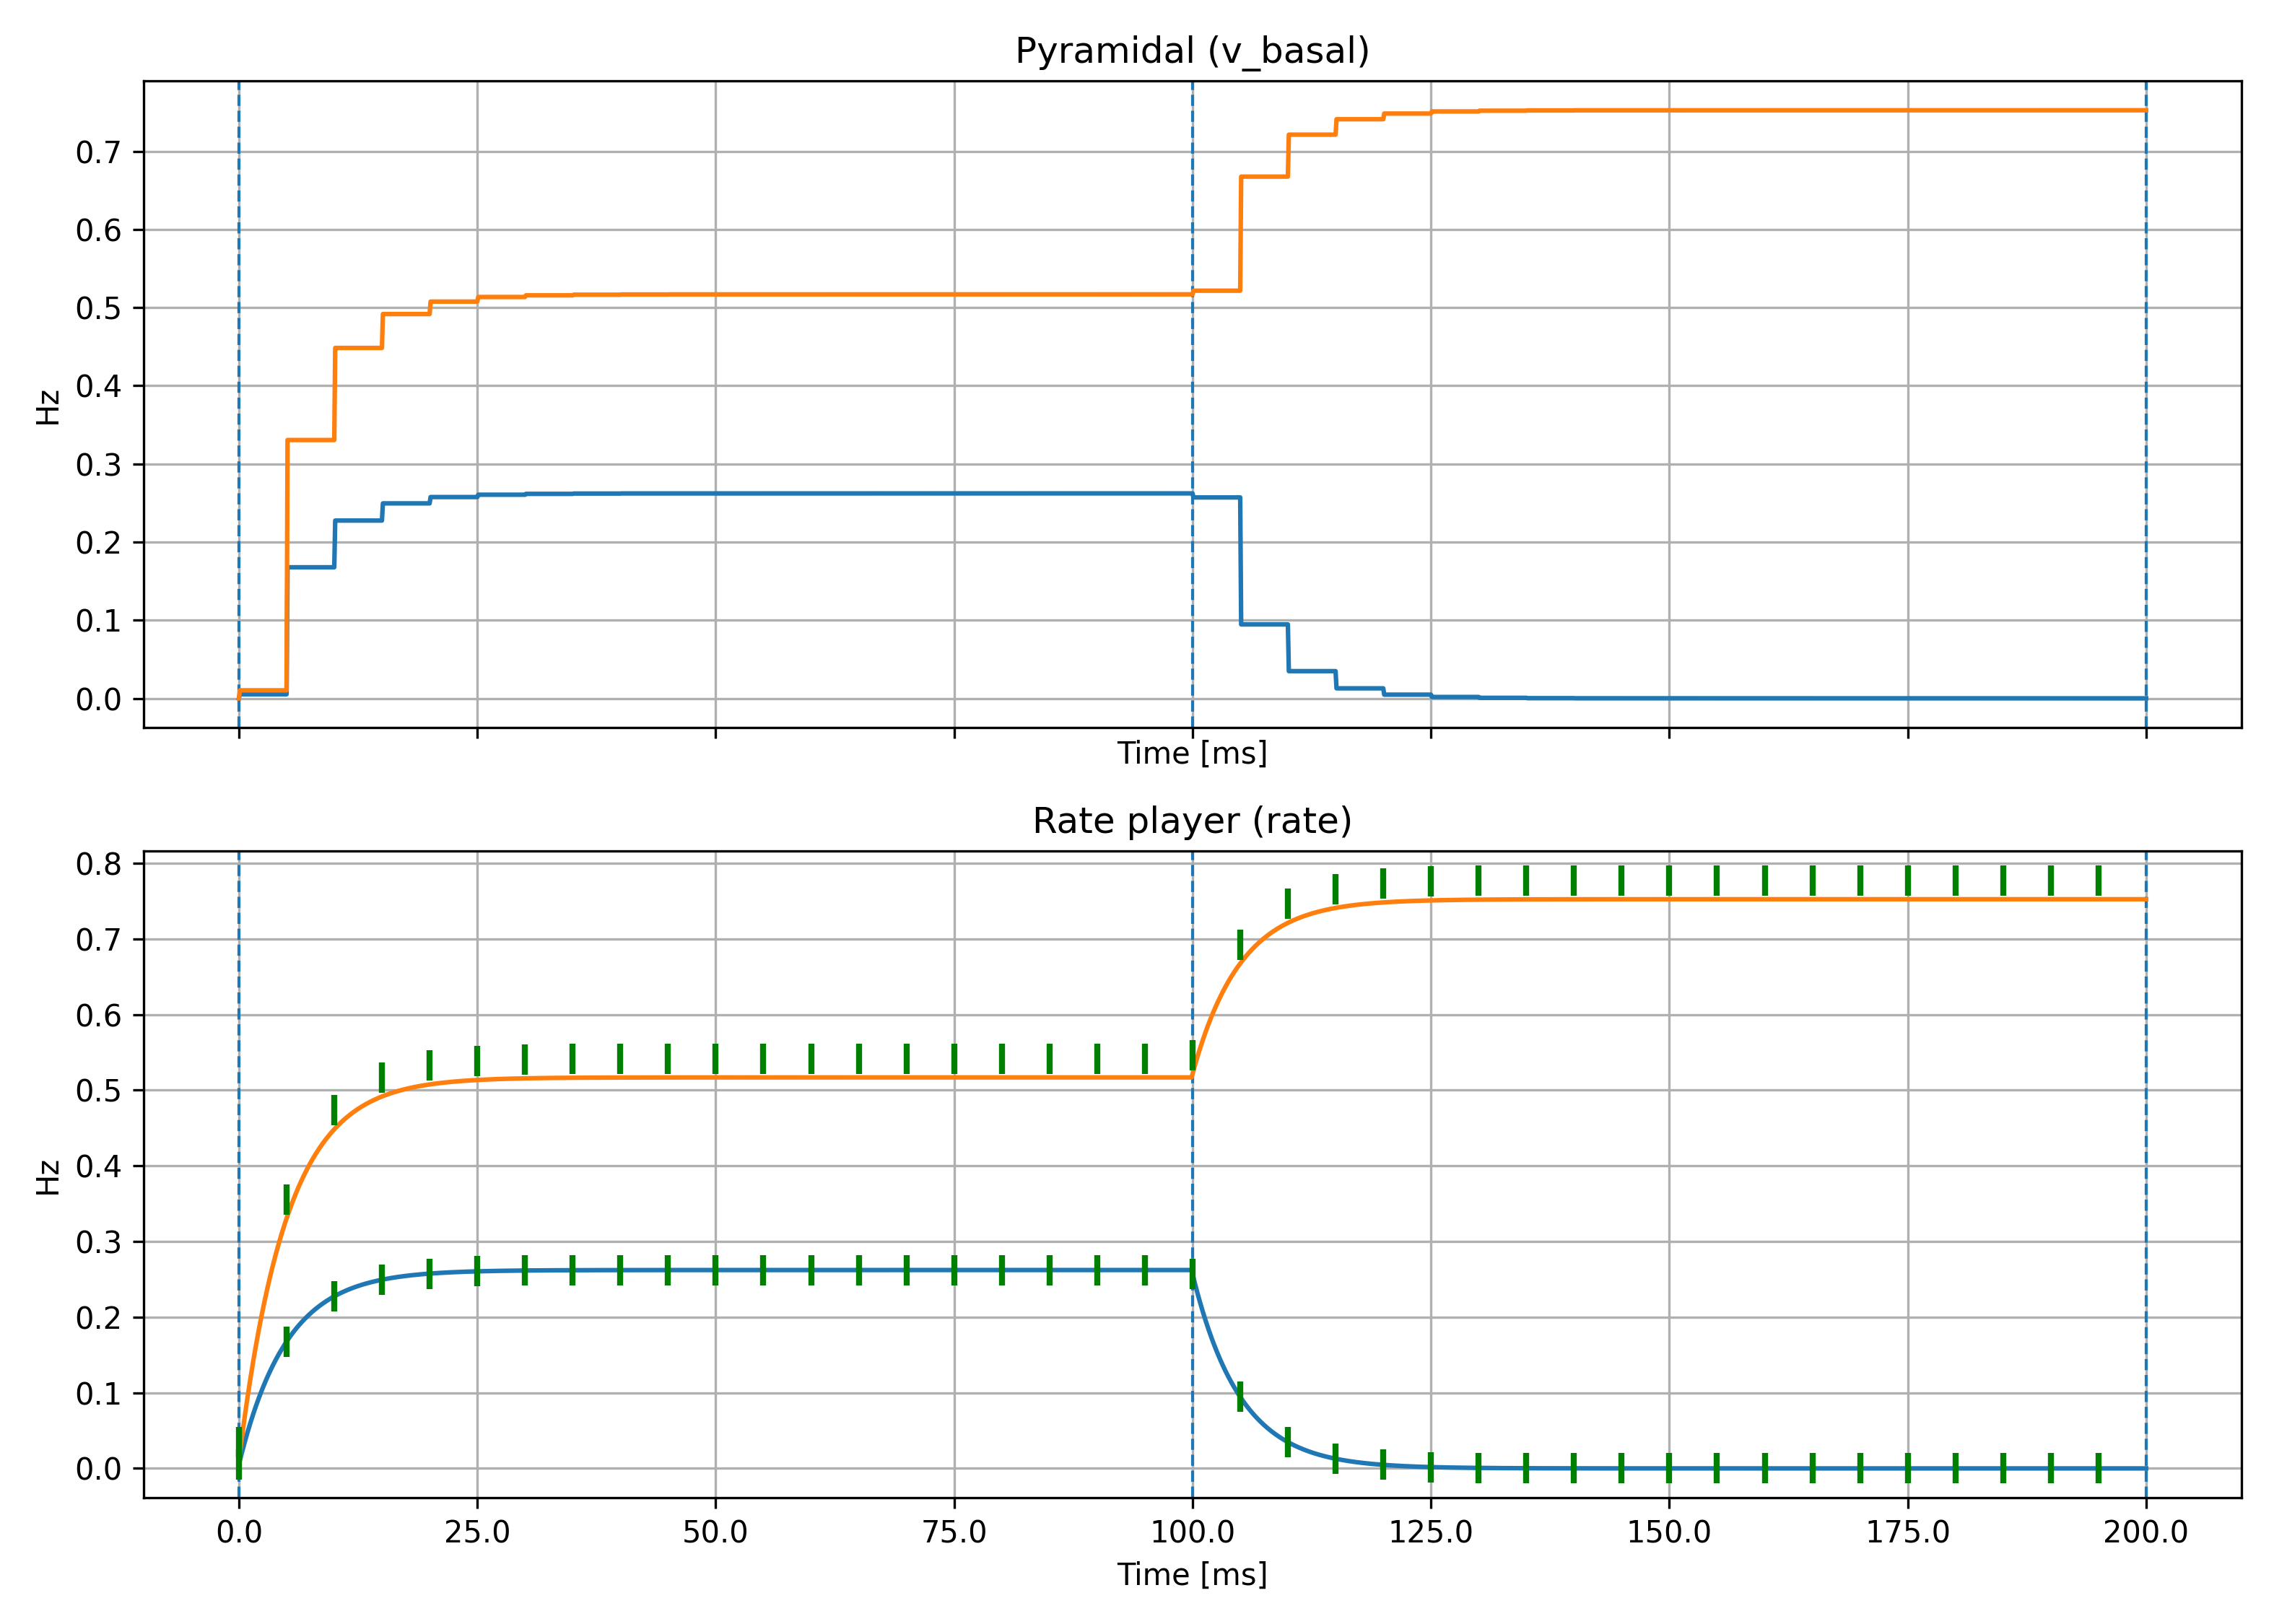
\includegraphics[width=\textwidth]{fixed_period_5_rate_player_plus_pyramid_behaviour.png}
        \caption{}
        \label{fig:fixed-period-transmission}
    \end{subfigure}
    % \hspace*{1cm}
    \hfill
    \begin{subfigure}[b]{0.35\textwidth}
        \centering
        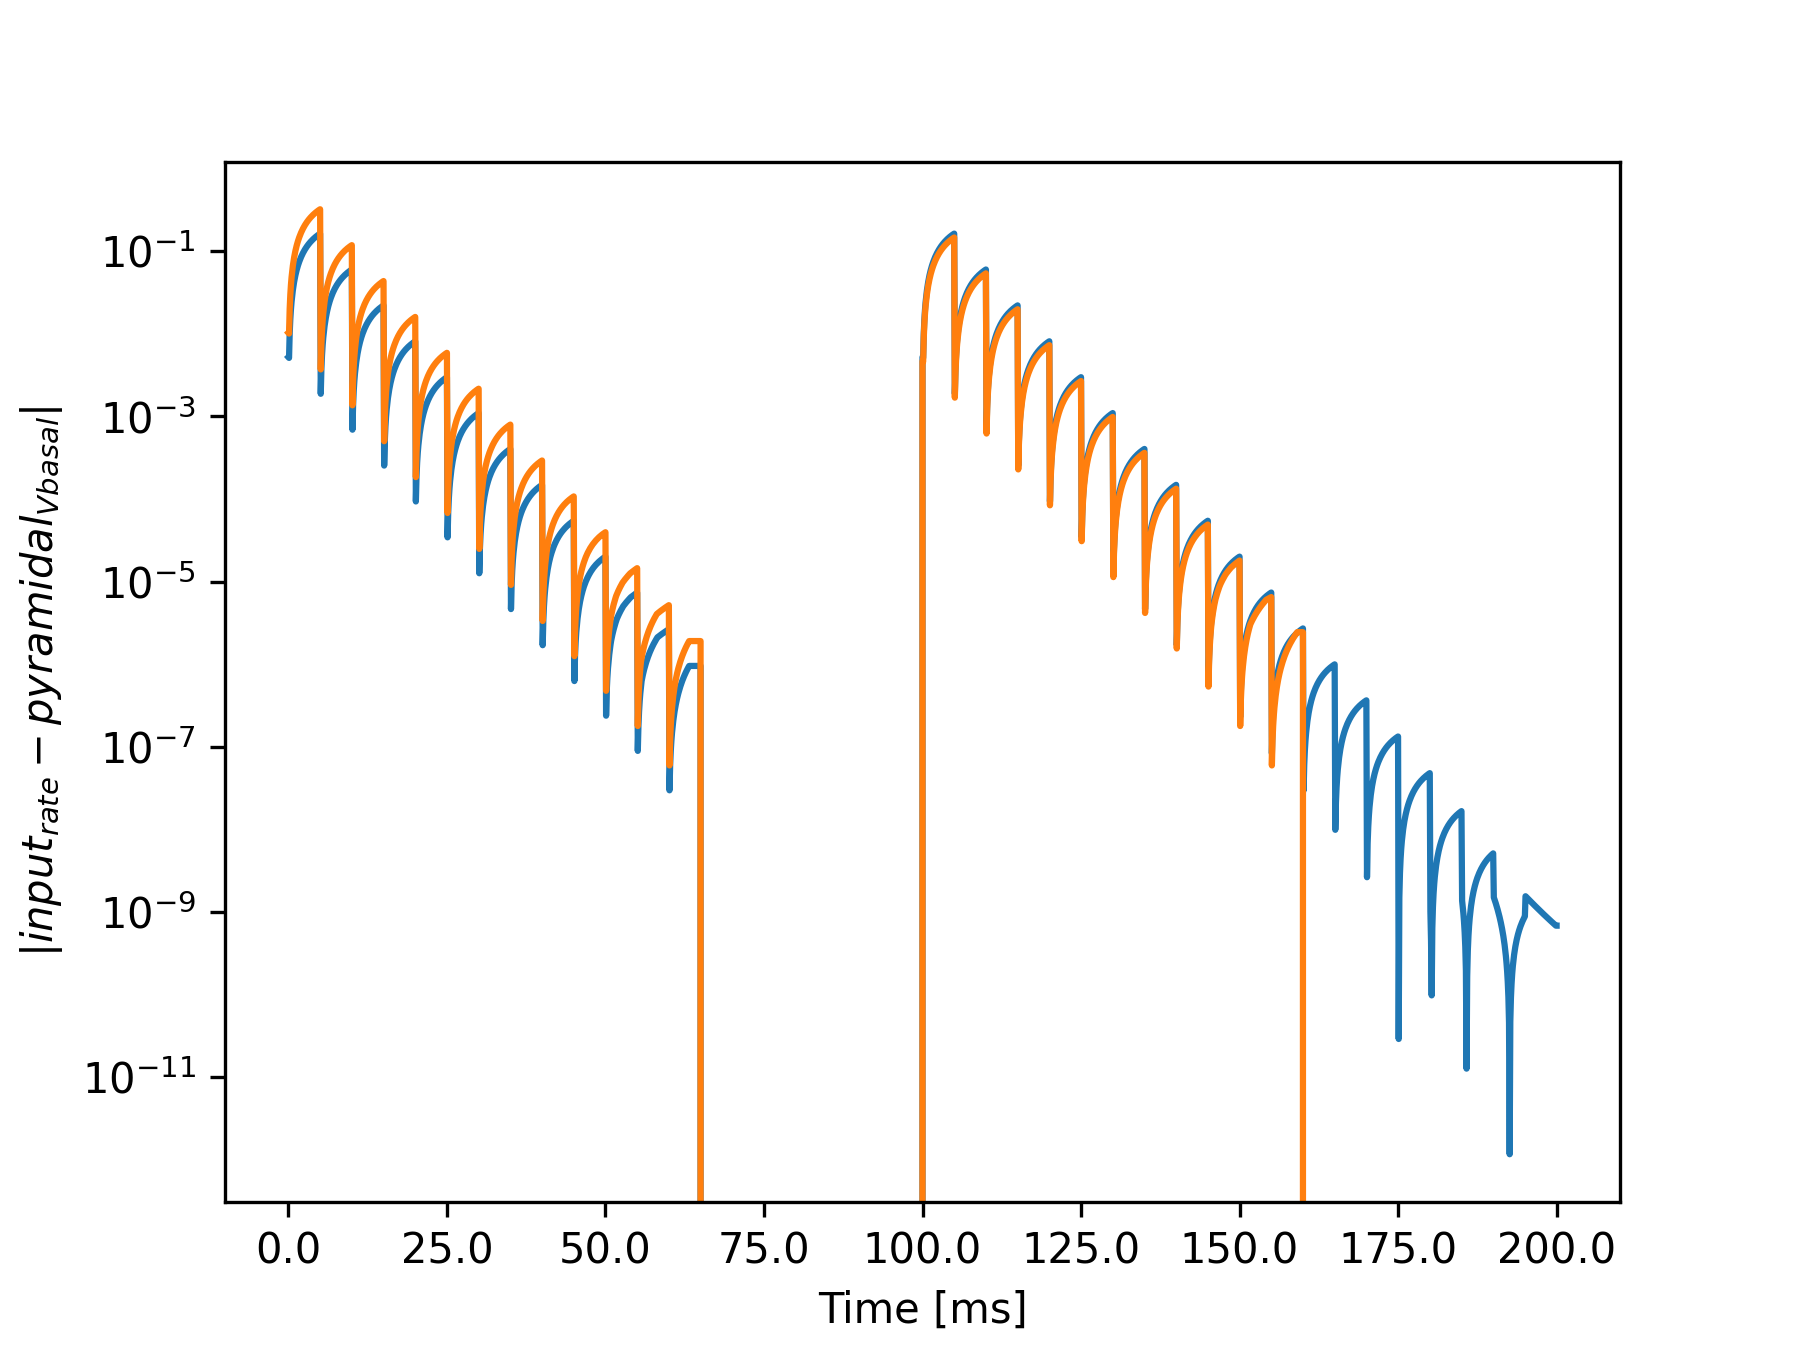
\includegraphics[width=\textwidth]{fixed_period_5_rate_differences.png}
        \vspace*{0.75cm}
        \caption{}
        \label{fig:fixed-period-signal-difference}
    \end{subfigure}
    \caption{Rate is transmitted with events emitted at a fixed interval.}
    \label{fig:fixed-period-rate-example}
\end{figure}

For the Yin Yang experiment, accuracy drops as the spiking period is increased (Figure~\ref{fig:accuracy-fixed-period})
Note that for $10 ms$ period the accuracy can go as high as with the $5 ms$ one, though the latter gets the top accuracy more consistently.


\begin{figure}[h!bt]
    \centering
    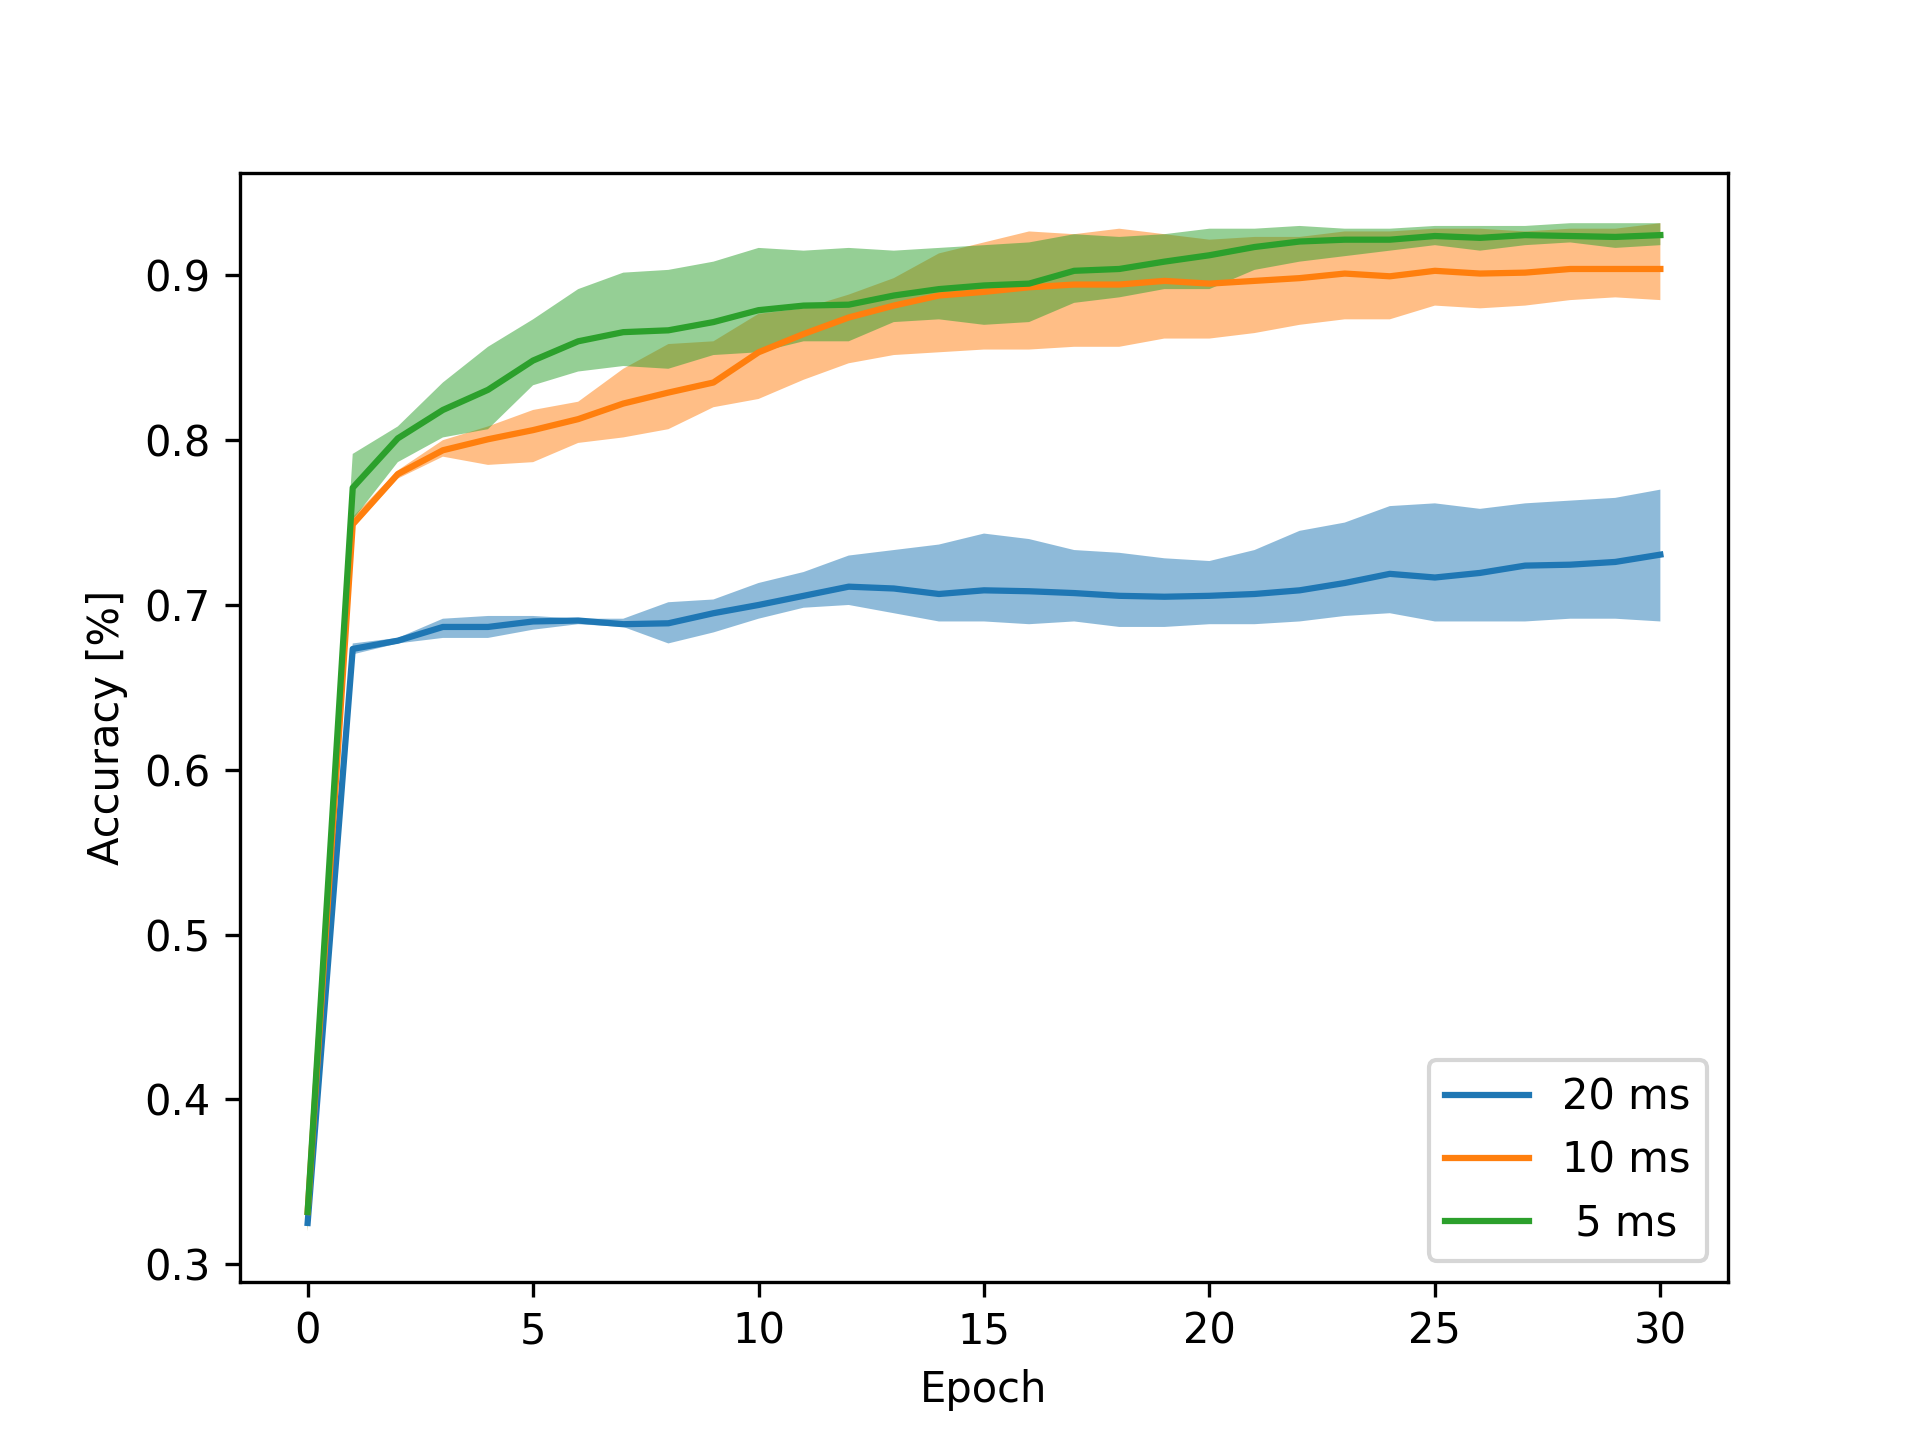
\includegraphics[width=0.6\textwidth]{accuracies_per_period_length.png}
    \caption{Accuracy drops as spike period length increases.}
    \label{fig:accuracy-fixed-period}
\end{figure}

I think this is because the teaching signal is arriving at the ``wrong'' time due to the delays introduced by the spiking signal Figure~\ref{fig:output-lag-vs-learning}.
\note{This could be fixed if we interleave the spiking start time per layer, though this may introduce more noise than needed}
\begin{figure}[h!bt]
    \centering
    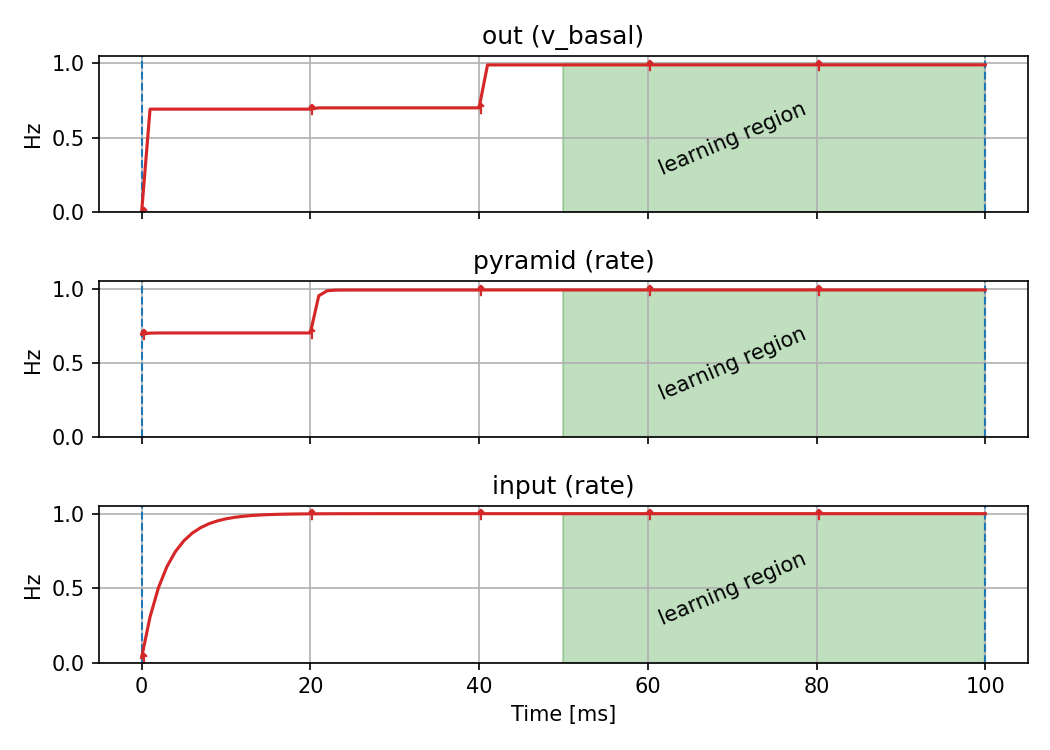
\includegraphics[width=0.6\textwidth]{rate_player_plus_pyramid_plus_inter_behaviour.png}
    \caption{Even in a feed-forward version, learning starts when output just arrived to }
    \label{fig:output-lag-vs-learning}
\end{figure}


\subsection{Rate Change}
When `outgoing' rates change and these changes are higher than a threshold, neurons emit events. \\
\note{this is largely inspired by the DVS emulation work I did before}
Since changes can be either positive or negatives, neurons emit 2 `types' of events (Figure~\ref{fig:rate-changes-events}.
\note{we currently send a payload so, effectively, there's only one event type}

\begin{figure}[h!bt]
    \centering
    \begin{subfigure}[b]{0.3\textwidth}
        \centering
        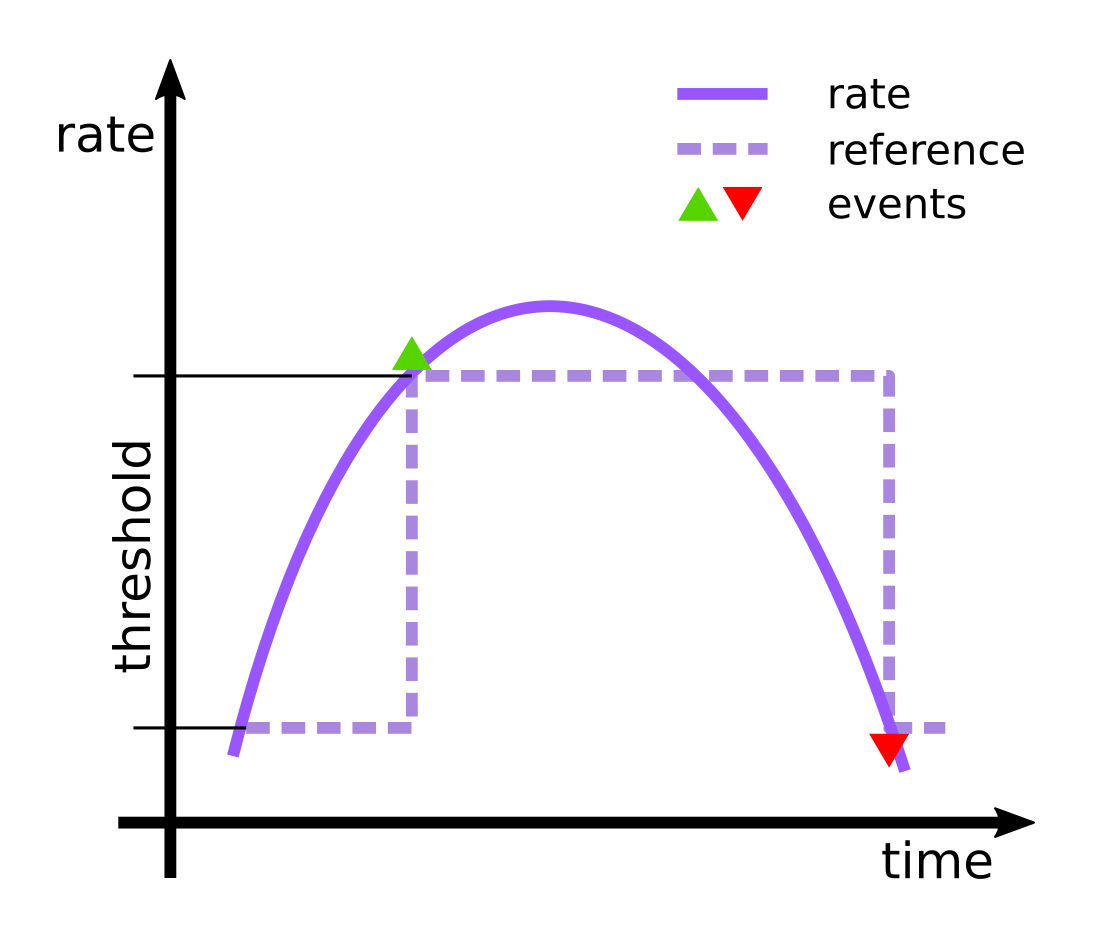
\includegraphics[width=\textwidth]{drate_events.png}
        \caption{}
        \label{fig:rate-changes-events}
    \end{subfigure}
    \hspace*{1.5cm}
    \begin{subfigure}[b]{0.3\textwidth}
        \centering
        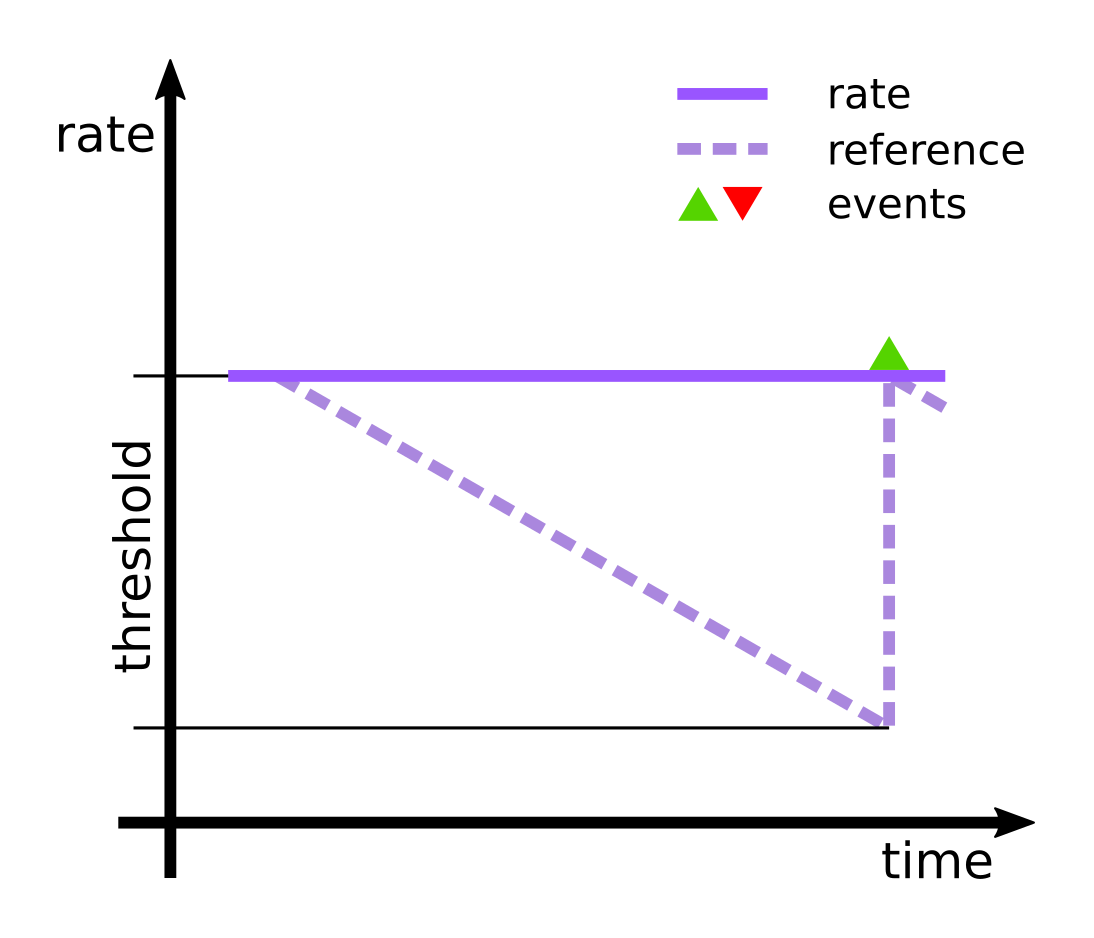
\includegraphics[width=\textwidth]{drate_decay_events.png}
        \caption{}
        \label{fig:rate-changes-decay}
    \end{subfigure}
    
    \caption{Rate changes generate events}
    \label{fig:rate-chagnes}
\end{figure}

Because in the stable phase of the simulation there are no rate changes and pre-synaptic spikes trigger weight changes, we added a decay to the reference value (Figure~\ref{fig:rate-changes-decay}). 
An example of the behaviour for this transmission scheme can be seen in Figure~\ref{fig:drate-transmission}.
Events are shown as vertical bars on top of the rate lines, we use green for positive rate changes and red for negative ones. 
\note{in the current implementation this is nothing but cosmetic as we use a payload to transfer the 'sign'}


\begin{figure}[h!bt]
    \centering
    \begin{subfigure}[b]{0.6\textwidth}
        \centering
        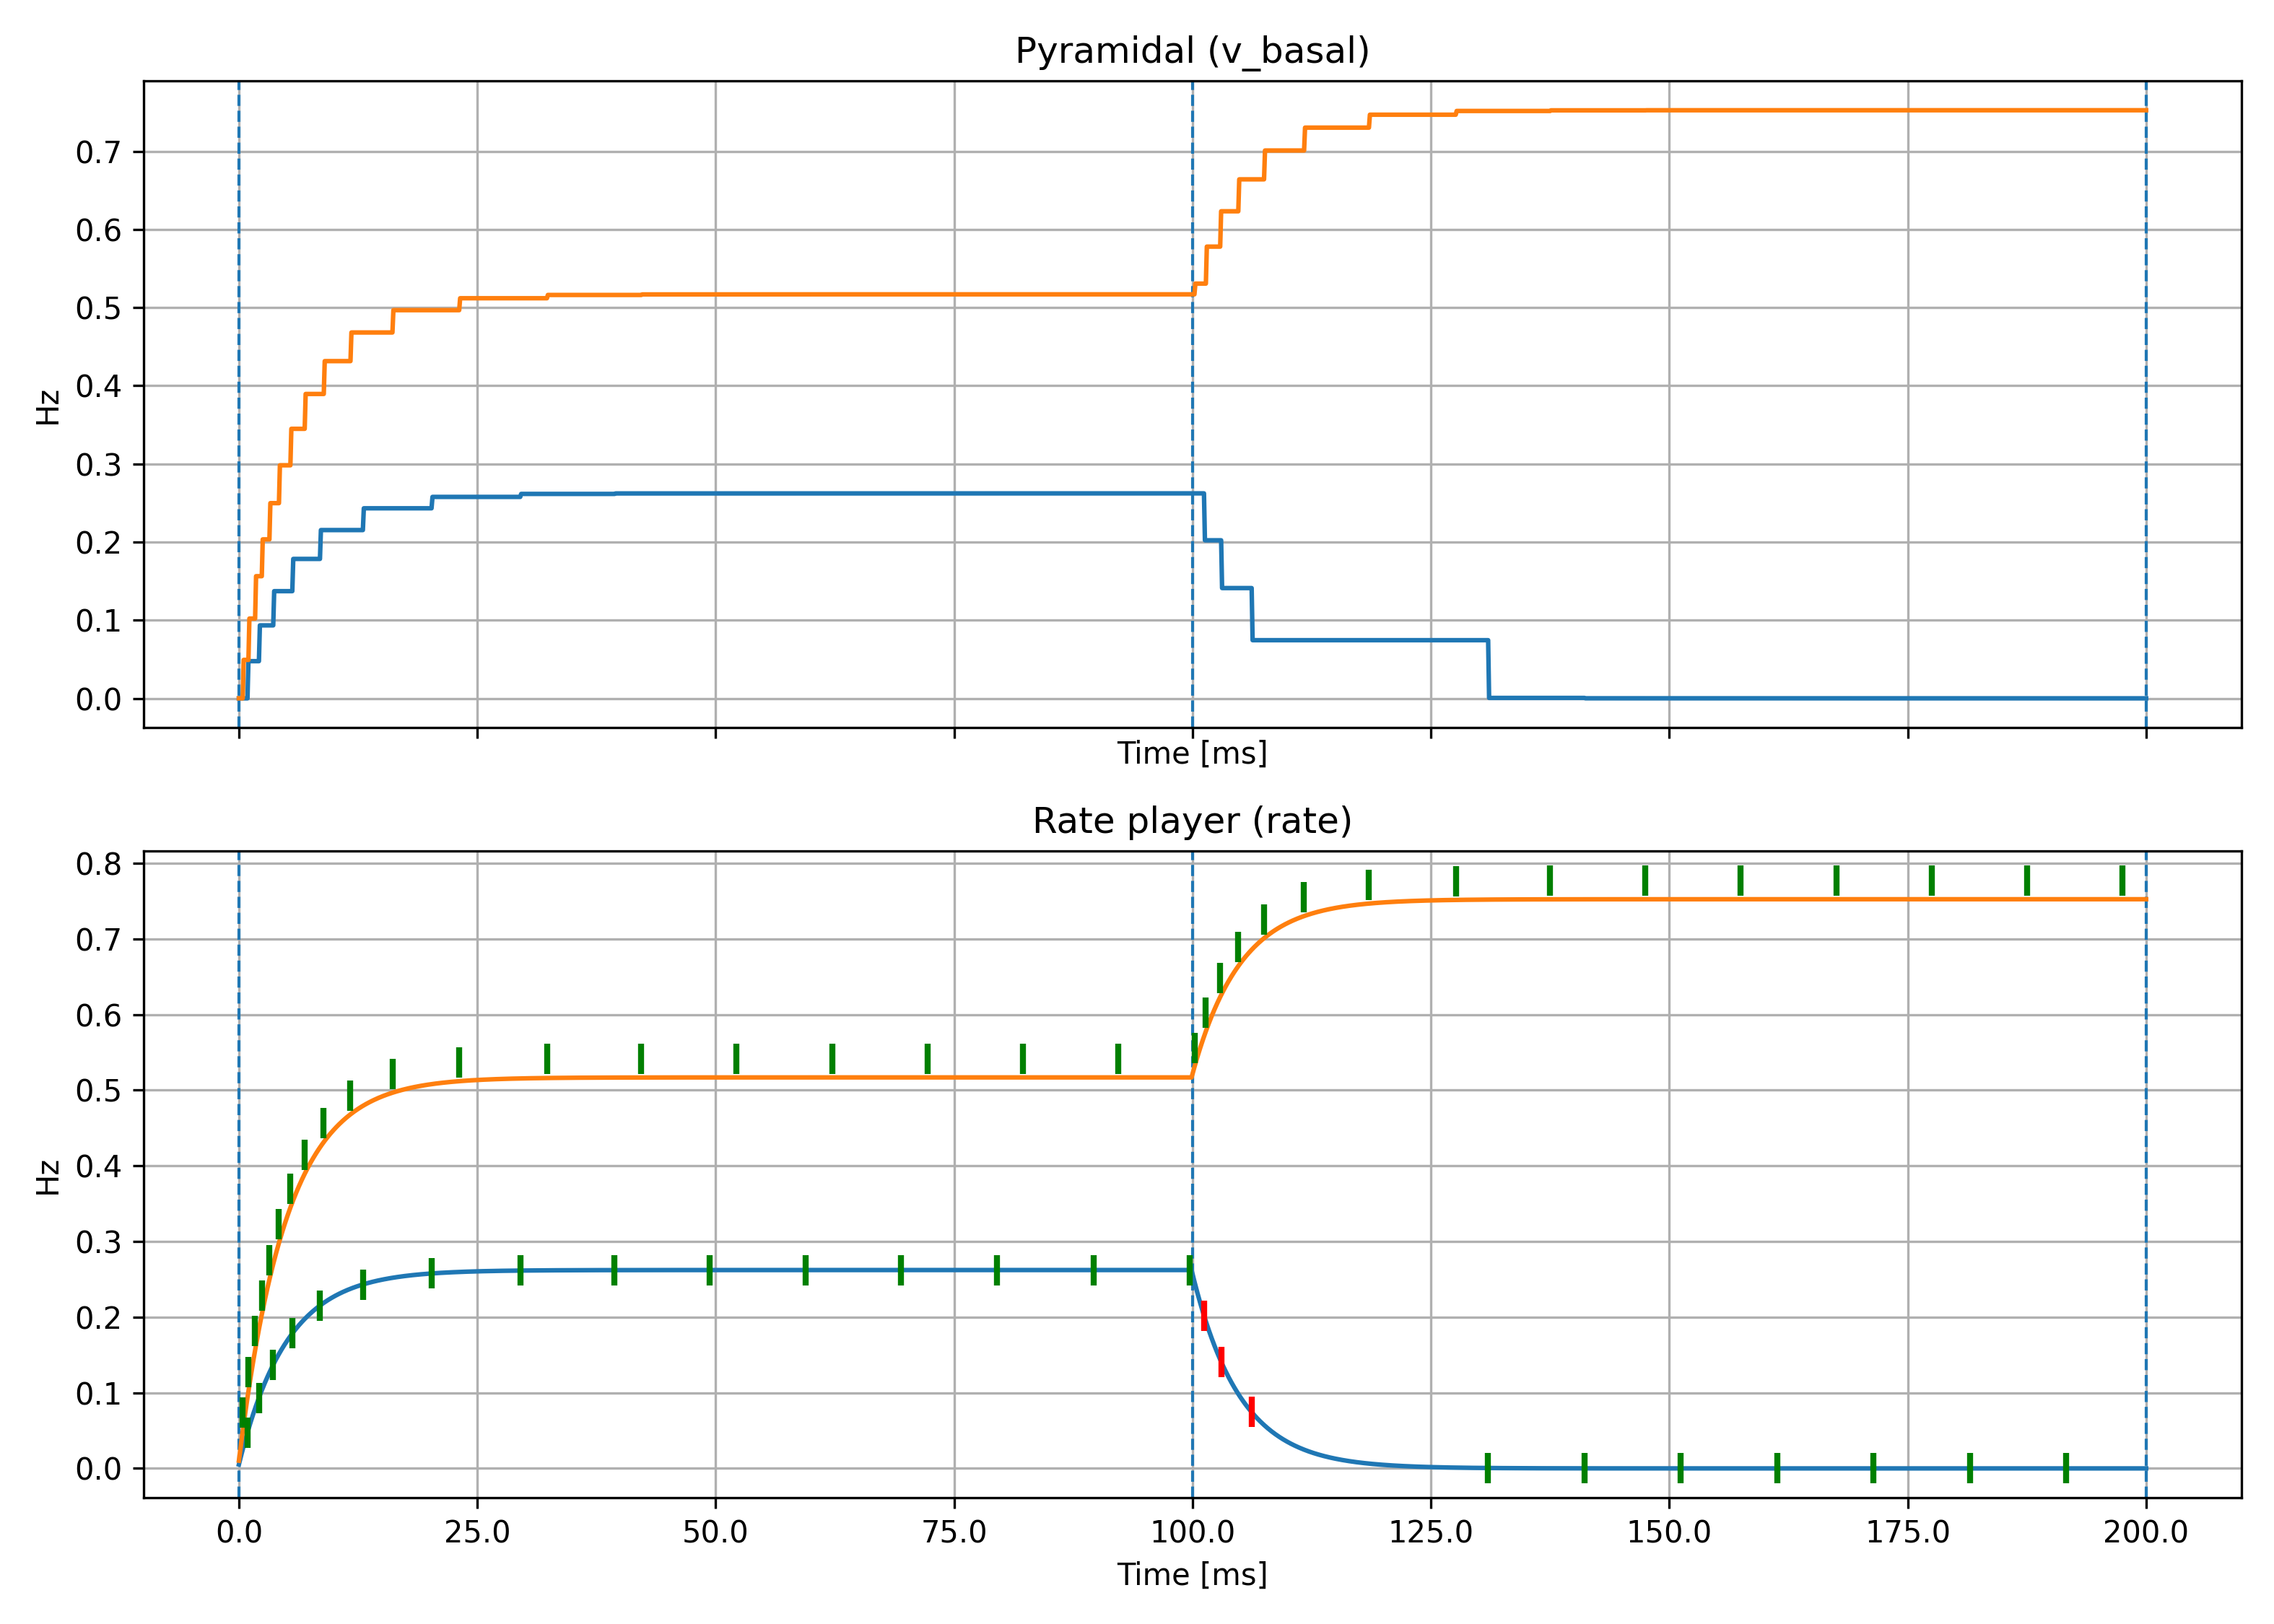
\includegraphics[width=\textwidth]{drate_0p05_rate_player_plus_pyramid_behaviour.png}
        \caption{}
        \label{fig:drate-transmission}
    \end{subfigure}
    % \hspace*{1cm}
    \hfill
    \begin{subfigure}[b]{0.35\textwidth}
        \centering
        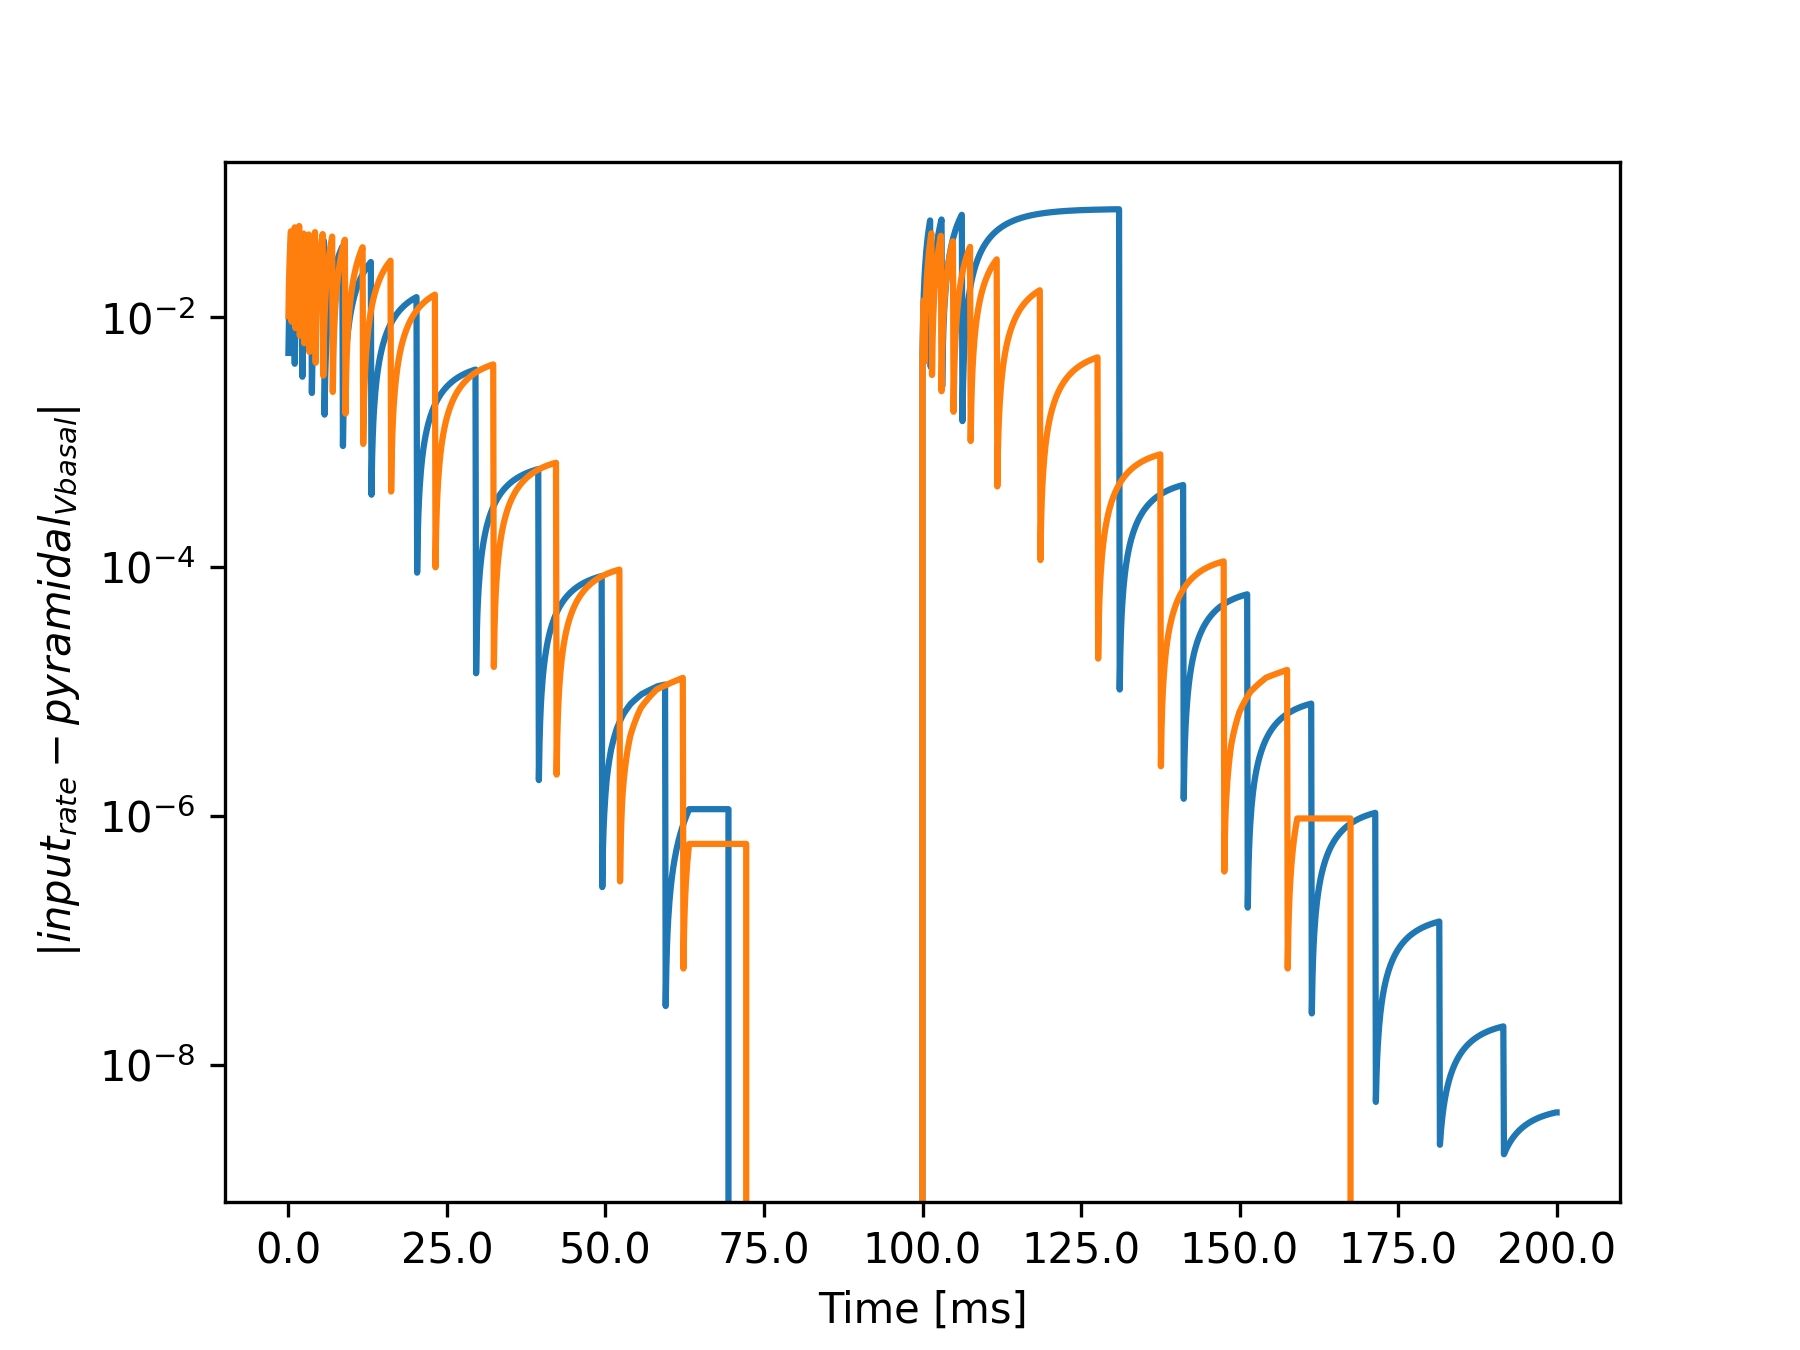
\includegraphics[width=\textwidth]{drate_0p05_rate_differences.png}
        \vspace*{0.75cm}
        \caption{}
        \label{fig:drate-signal-difference}
    \end{subfigure}

    \caption{Signal transmission through Rate-change triggered events, from input to Pyramidal basal compartment.}
    \label{fig:drate-example}
\end{figure}



\subsection{Perf analysis}

I expect that we can get some speed gains via event driven sims, yet to be measured\\
\note{Ah shit, I was super wrong!}\\
The profiling tools show that, as we increase the number of neurons, the compute time is spent mostly on synapse updates.\\
I am not 100\% sure but, my guess is that the overhead of spike processing (sorting/delivery/etc) plus a bit more complex maths starts to take a toll.\\
Another problem I see on the rate-change one, is that we can't probably should only use something like sigmoids to keep rate changes in a range that makes thresholds compatible. \\
\begin{figure}[!hbt]
    \centering
    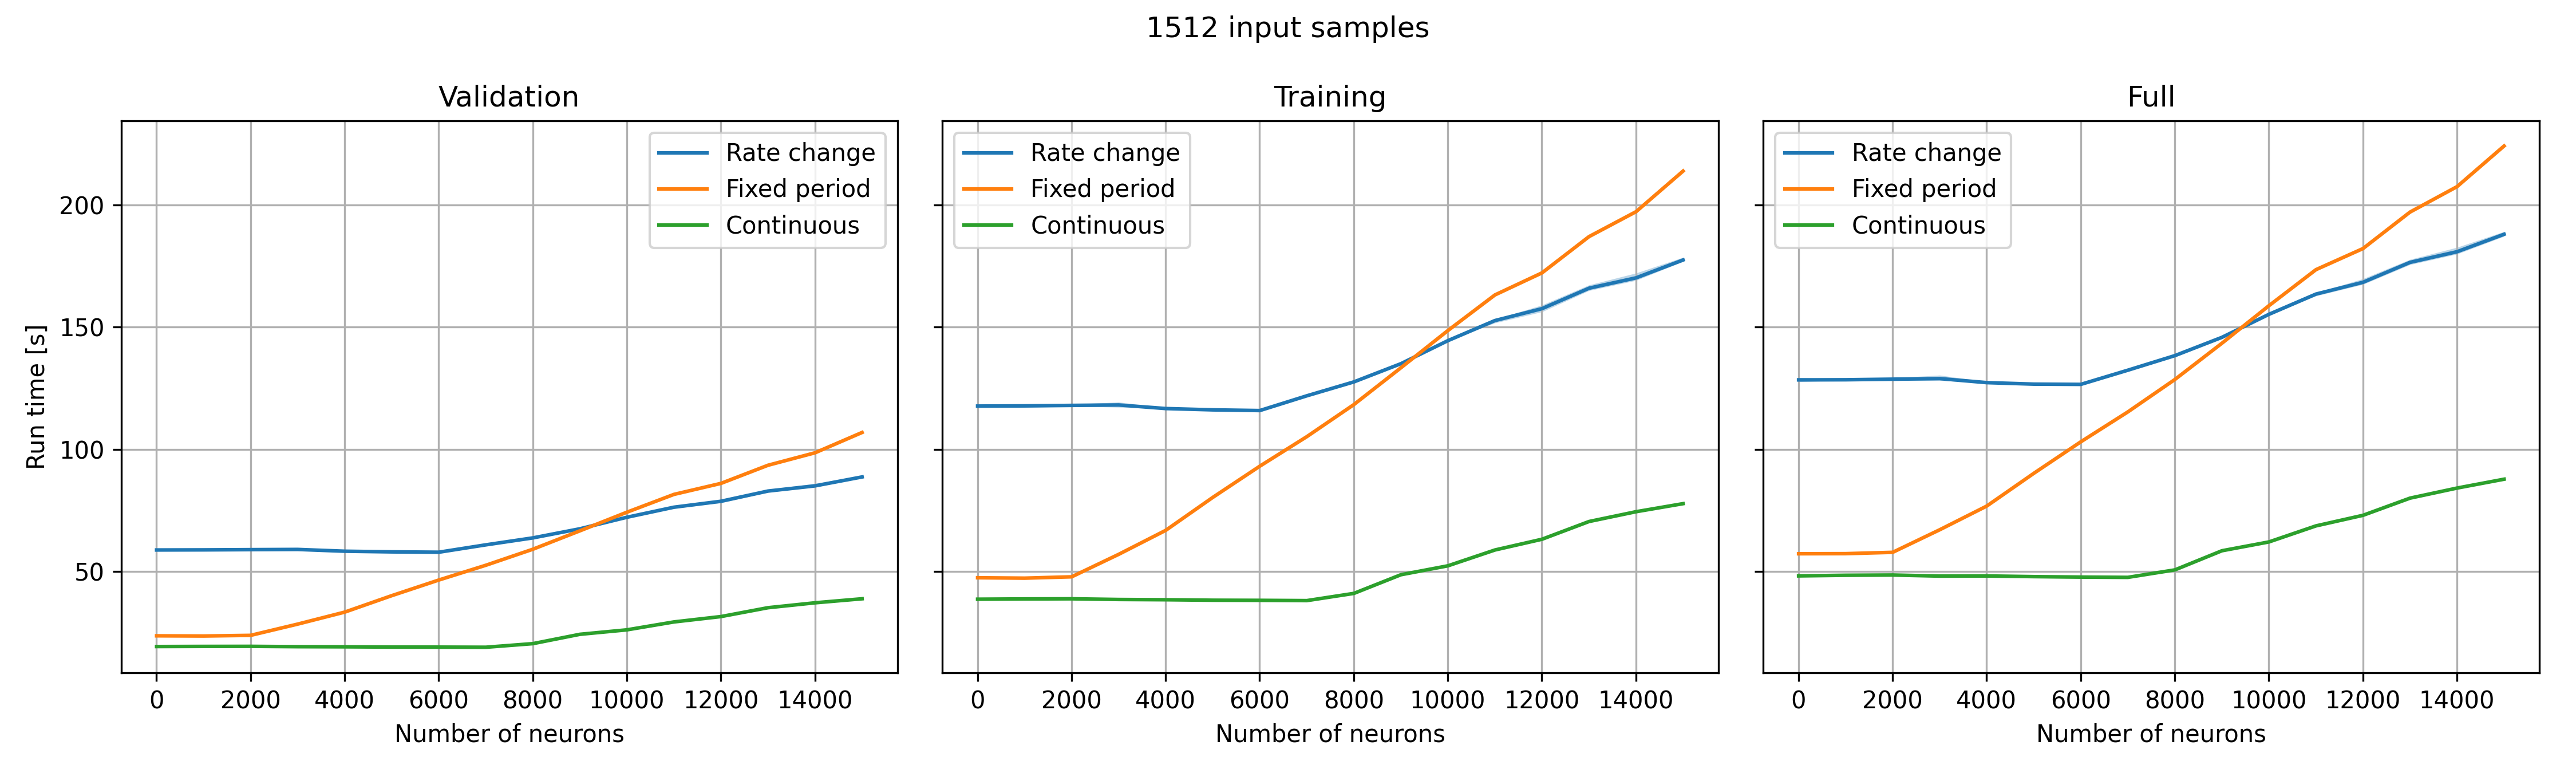
\includegraphics[width=0.7\textwidth,trim={0 0 12.2cm 1cm},clip]{perf_comparison_with_503_inputs.png}
    \caption{Time to run a training epoch on variations of the algorithm. Lower is better.}
    \label{fig:}
\end{figure}

\subsection{Not Working}
\subsubsection{Inter-spike interval}
Transmitting small values is a problem \\ 
Strategies to fix them, end up with evaluating synapses every time step or forcing a `learning' spike to when the learning region is active


\section{Conclusion}
Your conclusion here

\section*{Acknowledgments}
This was was supported in part by......

\appendix
\section{Extended Math}
For inter to pyramid synapse.
\subsection{First for Delta}
Here $V_{o}$ means voltage in the apical compartment for the post-synaptic neuron and $r_{i}$ the output rate (on the previous time step) for the pre-synaptic neuron.
\begin{eqnarray}
  \dot{\delta} = -\frac{1}{\tau}\left(\delta + V_{o} r_{i}\right)\\
  \dot{\delta} + \frac{1}{\tau}\delta = -\frac{1}{\tau} V_{o} r_{i}
\end{eqnarray}
This is a `standard' first-order ordinary differential equation so we use integrating factor $e^{t/\tau}$.
\begin{eqnarray}
  \dot{\delta}e^{t/\tau} + \frac{1}{\tau}\delta e^{t/\tau} &=& -\frac{1}{\tau} e^{t/\tau}V_{o} r_{i} \\
\end{eqnarray}
To fit into product rule for derivatives $\left[(f\cdot g)' = f\cdot g' + g\cdot f'\right]$
\begin{eqnarray}
f = e^{t/\tau} &\text{ and }& \dot{h} = \dot{\delta}\\
\dot{f} = \frac{1}{\tau} e^{t/\tau}  &\text{ and }& h = \delta
\end{eqnarray}
we now get
\begin{equation}
\left(\delta e^{t/\tau}\right)' = -\frac{1}{\tau} e^{t/\tau} V_{o} r_{i} 
\end{equation}
Integrating both sides
\begin{eqnarray}
\delta e^{t/\tau} &=& -V_{o} r_{i} \int_{0}^{t} \frac{1}{\tau} e^{t/\tau} dt \\
    &=& -V_{o} r_{i} \left[e^{t/\tau}\right]_{0}^{t} + C\\
    &=& -V_{o} r_{i} \left[e^{t/\tau} - 1\right] + C \\
\delta &=& \left[-V_{o} r_{i} \left(e^{t/\tau} - 1\right) + C \right] e^{-t/\tau}\\
\delta &=& -V_{o} r_{i} \left(1 - e^{-t/\tau} \right) + Ce^{-t/\tau}
\label{delta_at_t_with_C}
\end{eqnarray}
To find $C$ and, since we want to integrate between spikes, we'll calculate the constant at $t_k$ (last time at which pre-synaptic spiked). $\delta_k$ is the value of $\delta$ at time $t_k$.
\begin{eqnarray}
C &=& \left[\delta_k + V_{o} r_{i} \left(1 - e^{-t_k/\tau} \right)\right] e^{t_k/\tau}
\label{C_for_delta_at_k}
\end{eqnarray}
Substituting \ref{C_for_delta_at_k} in \ref{delta_at_t_with_C}

\begin{eqnarray}
\delta &=& -V_{o} r_{i} \left(1 - e^{-t/\tau} \right) + \left[\delta_k + V_{o} r_{i} \left(1 - e^{-t_k/\tau} \right)\right] e^{t_k/\tau}e^{-t/\tau}
\end{eqnarray}
Let $\Delta t = t - t_k$

\begin{eqnarray}
\delta &=& -V_{o} r_{i} \left(1 - e^{-t/\tau} \right) + \delta_k e^{-\Delta t/\tau}+ V_{o} r_{i} \left(e^{t_k/\tau} - 1\right)e^{-t/\tau}\\
\delta &=& -V_{o} r_{i} + \cancel{V_{o} r_{i} e^{-t/\tau}} + \delta_k e^{-\Delta t/\tau}+ V_{o} r_{i} e^{-\Delta t/\tau} - \cancel{V_{o} r_{i} e^{-t/\tau}}
\end{eqnarray}
Finally
\begin{eqnarray}
\delta &=& -V_{o} r_{i} \left(1 - e^{-\Delta t/\tau}\right)  + \delta_k e^{-\Delta t/\tau}
\end{eqnarray}

\subsection{Now for efficacy}
We'll use the same notation as before $V_{o} = V^{apical}_{post}$ and $r_{i} = r_{pre}$.
\begin{eqnarray}
	\dot{g} &=& \eta \delta \\
	\int\dot{g} &=& \eta \int\delta dt\\	
	g &=& \eta \int \left[ -V_{o} r_{i} \left(1 - e^{-\Delta t/\tau}\right)  + \delta_k e^{-\Delta t/\tau} \right]dt \\
	g &=& \eta \left[ -V_{o} r_{i} \left(t + \tau e^{-\Delta t/\tau}\right)  - \delta_k \tau e^{-\Delta t/\tau} \right] + C
	\label{eq:g-at-t}
\end{eqnarray}
Obtain the constant at time $t_k$, remember that $\Delta t = t - t_k$
\begin{eqnarray}
	C &=& g_{k} + \eta \left[ V_{o} r_{i} \left(t + \tau e^{-\Delta t/\tau}\right) + \delta_k \tau e^{-\Delta t/\tau} \right]\\
	C &=& g_{k} + \eta \left[ V_{o} r_{i} \left(t_{k} + \tau\right) + \delta_k \tau \right]
	\label{eq:gk}
\end{eqnarray}
Now substituting \ref{eq:gk} in \ref{eq:g-at-t}
\begin{eqnarray}
	g &=& \eta \left[ -V_{o} r_{i} \left(t + \tau e^{-\Delta t/\tau}\right)  - \delta_k \tau e^{-\Delta t/\tau} \right] +  \nonumber\\
	& & g_{k} + \eta \left[ V_{o} r_{i} \left(t_{k} + \tau\right) + \delta_k \tau \right]\\
	&=& g_{k} -\eta \left[V_{o} r_{i} \left(t_{k} + \tau - t - \tau e^{-\Delta t/\tau}\right)  -  \right. \nonumber\\
    & & \left. \delta_k \tau e^{-\Delta t/\tau} + \delta_k \tau\right] \\
	&=& g_{k} -\eta \left[V_{o} r_{i} \left(-\Delta t + \tau\left[1 - e^{-\Delta t/\tau}\right]\right)  +  \right. \nonumber\\
    & & \left. \delta_k \tau\left(1 - e^{-\Delta t/\tau} \right)\right]
\end{eqnarray}
Let $\gamma = 1 - e^{-\Delta t/\tau}$
\begin{eqnarray}
	g &=& g_{k} -\eta \left[V_{o} r_{i} \left(-\Delta t + \tau\gamma\right)  + 
          \delta_k \tau \gamma \right] \\
g &=& g_{k} -\eta \tau \left[V_{o} r_{i} \left(\gamma -\frac{\Delta t}{\tau} \right)  + 
\delta_k \gamma \right] 
\end{eqnarray}




\section{Weight change algorithms}
\subsection{Continuous}
% if ($(learning_on) > 0) {
%     scalar ddelta = $(integration_step_size) * (
%             -$(delta) + 
%             ( $(rate_post) - $(rate_basal_post) ) * $(rate_last_pre)
%     );
%     $(g) += DT * $(eta) * $(delta);

%     $(delta) += ddelta;
% }

% $(addToInSyn, $(g)*$(rate_pre));

\begin{algorithm}[h!tb]
\DontPrintSemicolon
\uIf{$LearningOn$}{
    $d\delta_{k} \gets AdjustedIntegrationStep * \left(-\delta_{k - 1} + PostComponent_{k - 1} * PreRate_{k - 2}\right)$\\
    $g_{k} \gets g_{k - 1} + IntegrationStep * \eta * \delta_{k - 1}$\\
    $\delta_{k} \gets \delta_{k} + d\delta_{k}$\\
}
\vspace*{0.5cm}
\Return $g_{k} * PreRate_{k-1}$

\end{algorithm}




\subsection{Event-driven}
% if ($(learning_on) > 0) {
%     scalar dt = $(t) - $(prev_sT_pre);
%     scalar edt = exp(-dt / $(tau));
%     scalar post_component = ($(rate_post) - $(rate_basal_post));
%     scalar _gamma = 1 - edt;
    
%     $(g) += $(eta) * $(tau) * ((dt / $(tau) - _gamma) * post_component * $(rate_last_pre) - $(delta) * _gamma)  ;
    
%     $(delta) = -_gamma * post_component * $(rate_last_pre) + edt * $(delta);
% }

% // compute input current after weight update
% $(addToInSyn, $(g)*$(rate_pre) - $(prev_val));
% $(prev_val) = $(g)*$(rate_pre);

\begin{algorithm}[h!tb]
\DontPrintSemicolon
\uIf{$LearningOn$}{
    $dt \gets t - PrePreviousSpikeTime$ \\
    $ExpDt \gets exp^{-dt / \tau}$ \\
    $\gamma \gets 1 - ExpDt$ \\

    $g_{k} \gets g_{k - 1} + 
        \eta * \tau * \left[\left(\frac{dt}{\tau} - \gamma\right) * PostComponent_{k - 1} * PreRate_{k - 2} - 
            \delta_{k - 1} * \gamma\right]$  
    
    $\delta_{k} \gets ExpDt * \delta_{k - 1} - \gamma * PostComponent_{k - 1} * PreRate_{k - 2}$
    
}
\vspace*{0.5cm}

$PreviousOutput_{k} \gets  g_{k} * PreRate_{k - 1}$\\
\Return $g_{k} * PreRate_{k-1} - PreviousOutput_{k - 1}$\\
\end{algorithm}

%Bibliography
\bibliographystyle{plainnat}  
\bibliography{references}  


\end{document}

